\documentclass[prb,preprint]{revtex4-1} 
% The line above defines the type of LaTeX document.
% Note that AJP uses the same style as Phys. Rev. B (prb).

\usepackage{amsmath}  % needed for \tfrac, \bmatrix, etc.
\usepackage{amsfonts} % needed for bold Greek, Fraktur, and blackboard bold
\usepackage{graphicx} % needed for figures
\usepackage{tabularx}

\begin{document}

\title{Superconductivity: \\Measuring Critical Temperatures of YBCO and BSCCO}
% In a long title you can use \\ to force a line break at a certain location.

\author{Jiajun Shi}
\email{jshi15@amherst.edu} 
\affiliation{Department of Physics, Amherst College, Amherst, MA 01002}
\author{He Claudia Yun}
\email{hyun@smith.edu}
\affiliation{Department of Physics, Smith College, Northampton, MA 01063}

% See the REVTeX documentation for more examples of author and affiliation lists.

\date{\today}

%____________abstract____________________________________________

\begin{abstract}
The phenomenon of superconducting was first discovered in 1911, and has been a popular research field ever since due to its great utility. A key property of a superconductor is its critical temperature, the temperature at which its resistance suddenly drops to zero. In this lab, we measured the critical temperatures of two kinds of superconductors: $YBa_{2}Cu_{3}O_{7}$ (YBCO) and $Bi_{2}Sr_{2}Ca{2}Cu_{3}O_{9}$ (BSCCO). We cooled the prepared devices, including superconductor samples, thermocouples, current probes and voltages probes, down to as low as 85K with liquid nitrogen, and recorded their resistances and temperatures during the cooling and heating process. For YBCO, we also used different currents to test the current dependency of its critical temperature. Igor Pro was used to analyze the data. The critical temperature of YBCO is found to range from 109.5K to 119.4K, with no obvious evidence of current dependency. However, the uncertainty in the critical temperature for YBCO is 50\% on average, which is too high to reach any solid conclusion. The critical temperature for BSCCO is found to be $116\pm6$K, which is consistent with the expected value of 110K within uncertainty.\\

\end{abstract}

\maketitle 

%____________Introduction____________________________________________
\section{Introduction}

In 1911, Dutch physicist Kamerlingh Onnes studied the electrical resistance of materials at very low temperature. He immersed a wire made of solid mercury in liquified helium (4.2K), and observed that the resistance of the wire abruptly dropped to zero. This led to the discovery of superconductivity, the phenomenon that certain material's electrical resistance vanishes at a temperature called the critical temperature. The critical temperature is material-dependent, and usually ranges between 1K and 20K for ordinary superconductors such as solid mercury or lead.\\

Normally, when an electron passes through a crystal lattice, the atoms collide with the electron, hindering its motion. This process decreases the rate of flow of electrons, and is thus the origin of electrical resistance. Historically, it is sometimes postulated that at absolute zero temperature, electrons cannot go through crystal lattice at all, which means the electrical resistance becomes infinite at 0K. Fig. \ref{phonon} shows an electron passing through a crystal lattice in non-superconducting phase. Physicists did not reach a conclusion about the mechanism behind superconductivity until 1957, when John Bardeen, Leon Cooper, and John Schrieffer ("BCS") proposed the BCS theory. The BCS theory characterizes superconductivity as a quantum mechanical phenomenon-- as an electron passes through the material, it attracts nearby positive charges in the lattice, causing a deformation of the lattice, and creating a local area of positive charges.This positively charged region will attract another electron with spin opposite to the first one to move into the region and pair with the first electron. It is true that ,ordinarily, the direct interaction between two electrons is the repulsive Coulomb force. However, inside a low-temperature superconductor, the coupling of electrons to the lattice introduces another attractive interaction that can overcome the Coulomb interaction, pairing the two electrons together, as shown in Fig. \ref{superconducting}. The electron pair is called a Cooper pair. Now, as many electrons pass through the material, there will be many such electron pairs present, forming a condensation area with high density. The condensation of electron pairs increases the energy required to cancel any single pairing in the condensate, meaning that the oscillating atoms in the lattice need to give up more energy to affect the motion of any electron pair. At sufficiently low temperatures (below the critical temperature), the oscillation energy of the atoms decreases below the energy required to break electron pairs. Thus, the electron pair condensate can flow through the lattice while experience no resistance at all.\\

\begin{figure}[h]
\centering
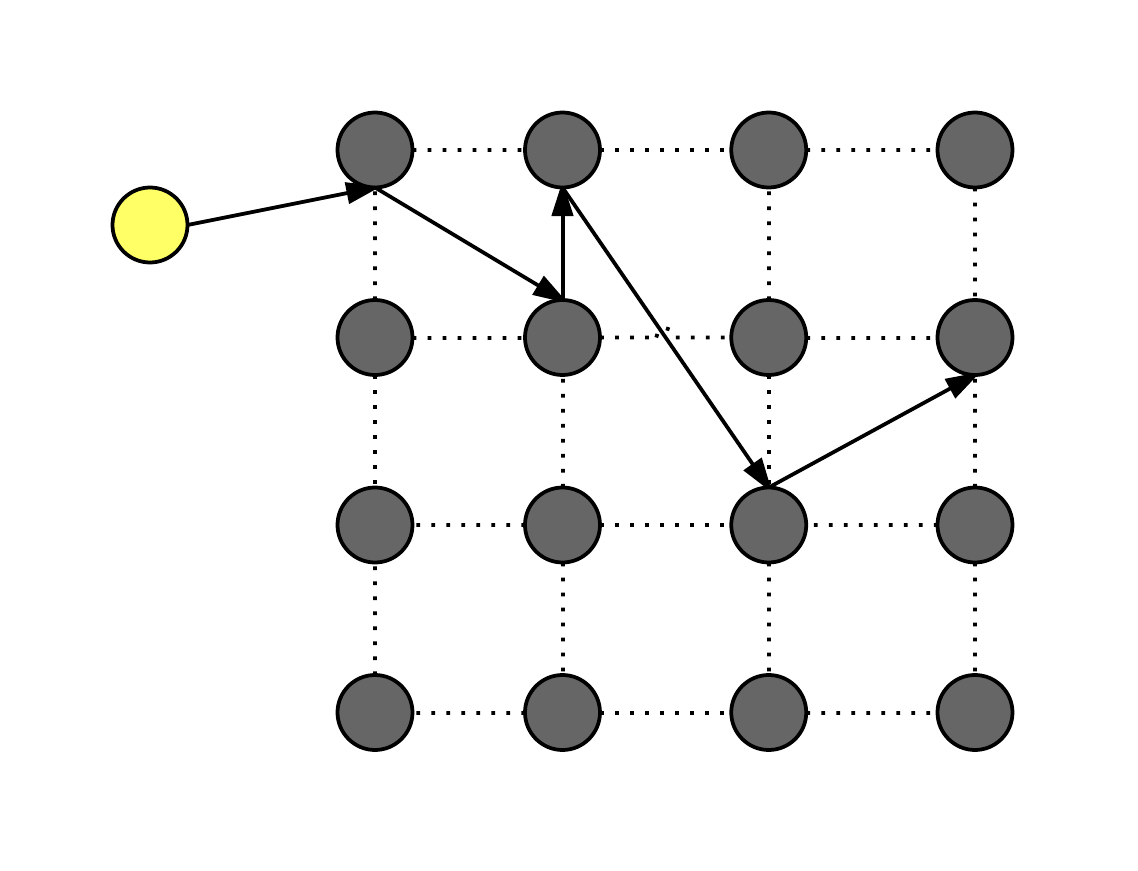
\includegraphics[width=\textwidth]{phonon.png}
\caption{Electron colliding with the atoms in the lattice under non-superconducting state.}
\label{phonon}
\end{figure}

\begin{figure}[h]
\centering
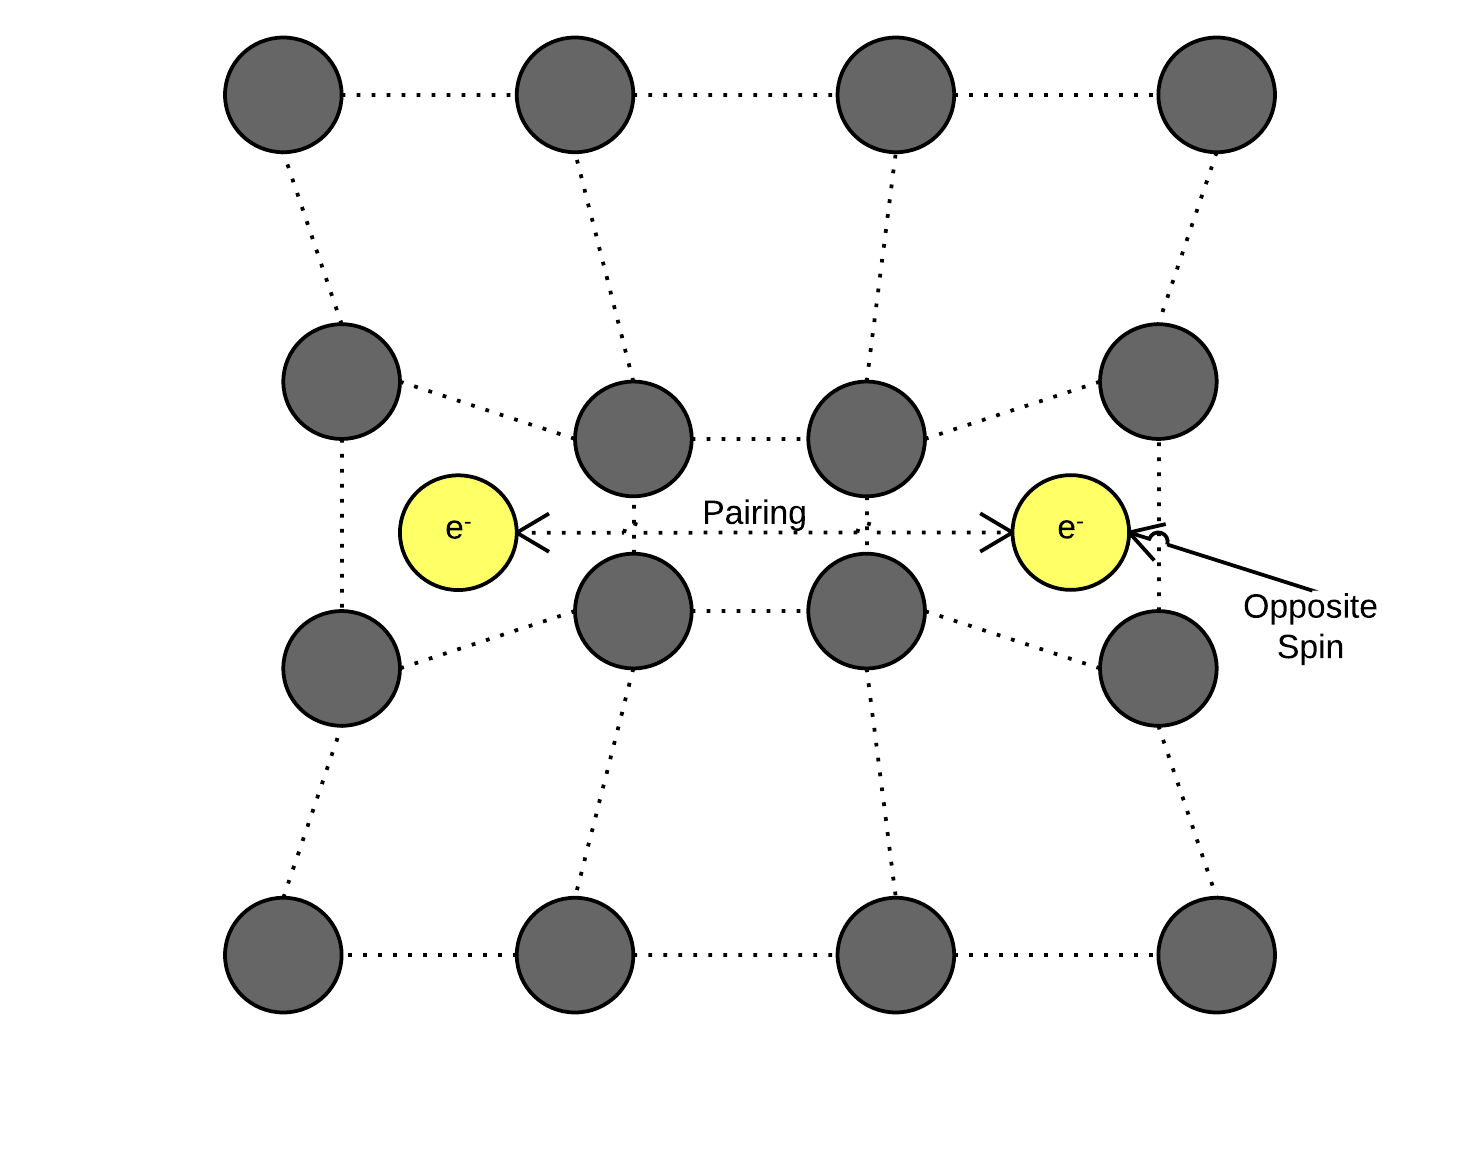
\includegraphics[width=\textwidth]{superconducting.png}
\caption{Two electrons form a Cooper pair due to electron-lattice coupling. The coupled electrons can together move through the lattice with no resistance.}
\label{superconducting}
\end{figure}


After the initial discovery of the superconductivity effect, physicists continued to seek materials with higher critical temperatures. Until now, there are only few materials that are known to have critical temperatures higher than the boiling point of liquid nitrogen (77K). These materials are categorized as high-temperature superconductors. The first superconductor discovered with critical temperature higher than 77K is yttrium barium copper oxide, $YBa_{2}Cu_{3}O_{7}$ (YBCO), which has an experimentally observed critical temperature of around 92K. Another notable example is bismuth strontium calcium copper oxide, $Bi_{2}Sr_{2}Ca{2}Cu_{3}O_{9}$ (BSCCO), which has three superconducting phases due to its structure. The three phase transitions occur at 20, 85, and 110K. The existence of high-temperature superconductors allow for more cost-efficient superconducting schemes, as liquid nitrogens can be relatively easy to mass produce. It is worth noting that although the BCS theory was successful in explaining low-temperature superconductivity, it cannot be generalized for high-temperature superconductors-- the mechanism behind high-temperature superconductivity is yet to be discovered. \\

The zero-resistance property of superconductors is utilized in many scientific applications. Since there is no energy loss for electrons due to their collisions with the atoms, a loop of superconducting wire can support an ever-lasting electric current with no external power supply, as in Fig. \ref{loop}. By Ohm's law, $I=V/R$, the current inside a superconducting wire is extremely large even with a relatively small voltage. This property allows us to generate strong magnetic field by superconducting electromagnets, which are widely used in magnetic resonance imaging, nuclear magnetic resonance, electromagnetic particle accelerators, etc.\\

\begin{figure}[h]
\centering
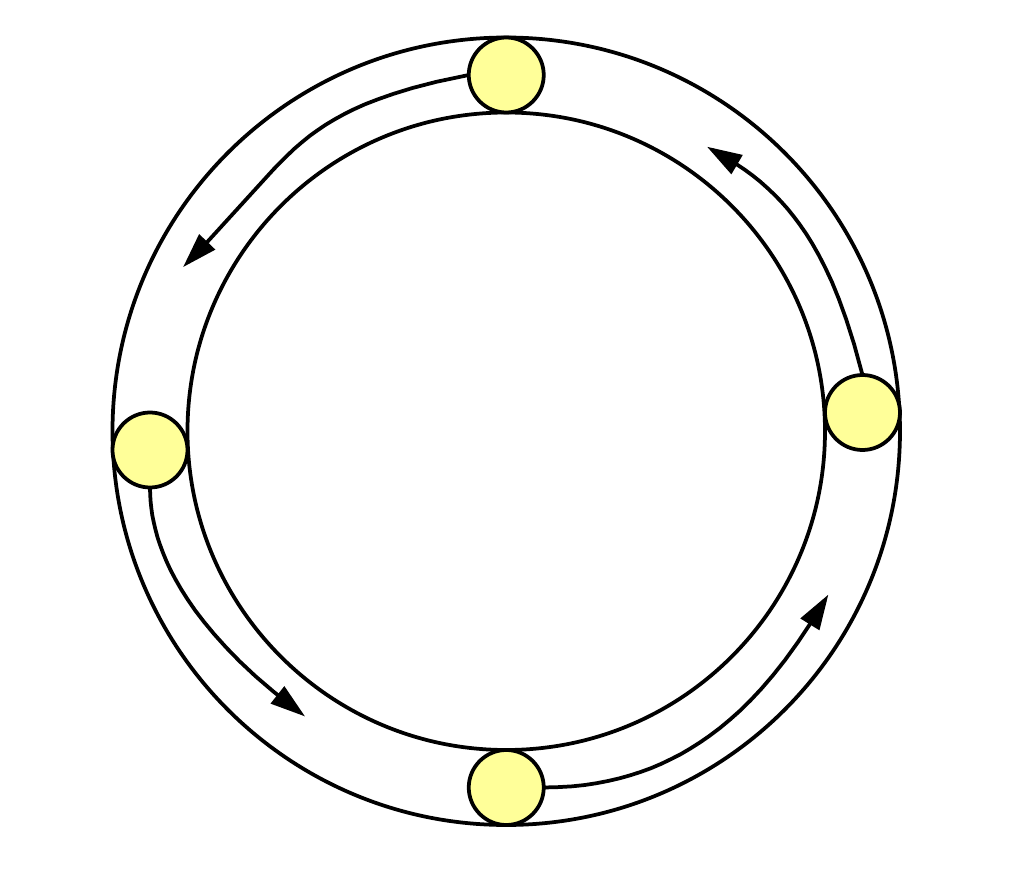
\includegraphics[width=70mm]{loop.png}
\caption{A loop of perfectly superconducting wire allows the flow of the electrons inside it to persist.}
\label{loop}
\end{figure}

We aim to reproduce the superconducting effect in the lab and measure the critical temperature. The only cooling method that is available to us is liquid nitrogen, so we are limited to the high-temperature superconducting materials. We will cool a sample of YBCO and another sample of BSCCO down using liquid nitrogen, and measure the resistance's dependence on temperature. For the YBCO sample, we will use a DC supply and a multimeter to determine the resistance of the material at a certain temperature. We will perform this measurement four times, each time with a current of different value flowing through the YBCO sample. Measuring the temperature requires the use of a thermocouple consisting of two dissimilar conducting materials connected together, which creates a temperature-dependent potential difference across the junction. With the calibration data of the thermometer, we can determine the temperature of the superconducting sample by measuring the voltage across the thermometer. For the BSCCO sample, we employ a lock-in amplifier feeding off a reference signal to eliminate the noise resulted from wire imperfections. The resistance's dependence on temperature for both samples is collected and imported into computer. We then determine the critical temperatures of the two materials using the collected data.\\


%____________Experiment____________________________________________
\section{Experiment}
Temperature and resistance are measured for two different materials: $YBa_{2}Cu_{3}O_{7}$ (YBCO) and $Bi_{2}Sr_{2}Ca_{2}Cu_{3}O_{9}$ (BSCCO). The experiments are done in two different ways for different materials.\\
\subsection{YBCO}
The setup of YBCO experiment is shown in the Fig. \ref{setup}. The device (Fig. \ref{sample}), including the YBCO sample, a thermocouple, a current probe and a voltage probe, is put in a plastic-foam cup and immersed in sands, which serve as insulator. The box variable resistor in Fig. \ref{setup} is only used for keeping the free wires at a fixed place. \\

\begin{figure}[h]
\centering
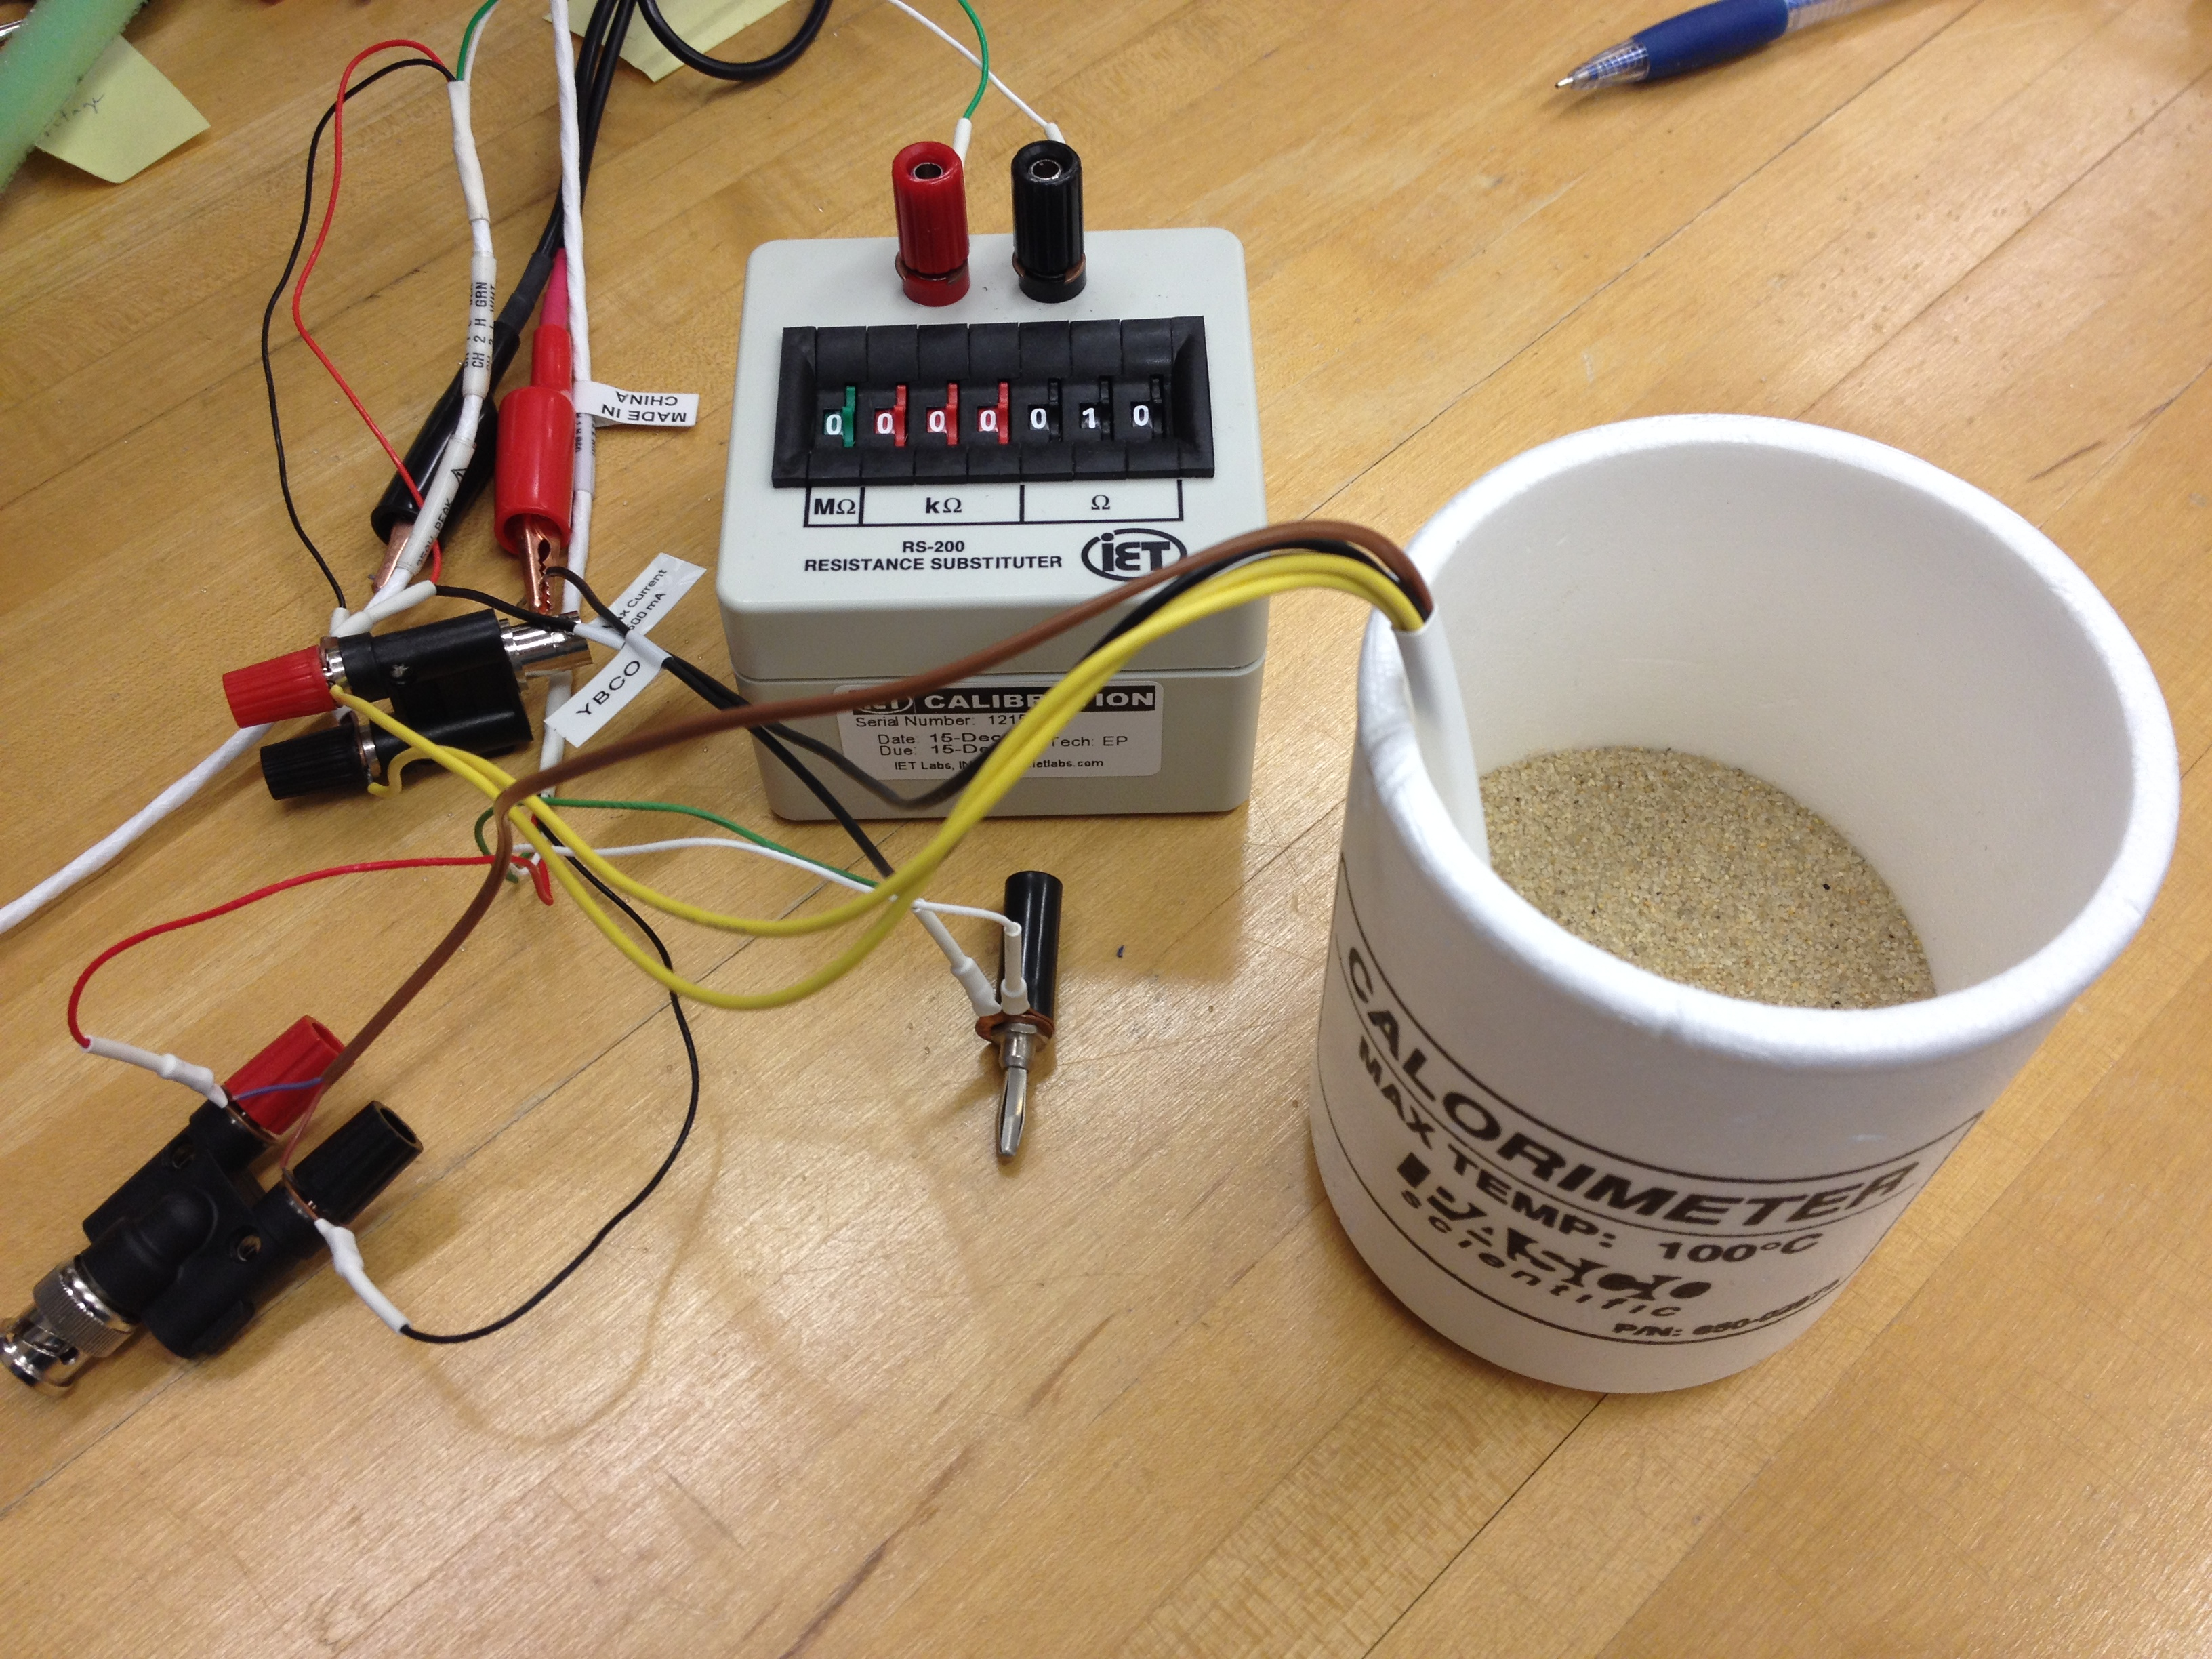
\includegraphics[width=14cm]{ybcosetup.jpg}
\caption{Picture of the experiment setup}
\label{setup}
\end{figure}

\begin{figure}[h]
\centering
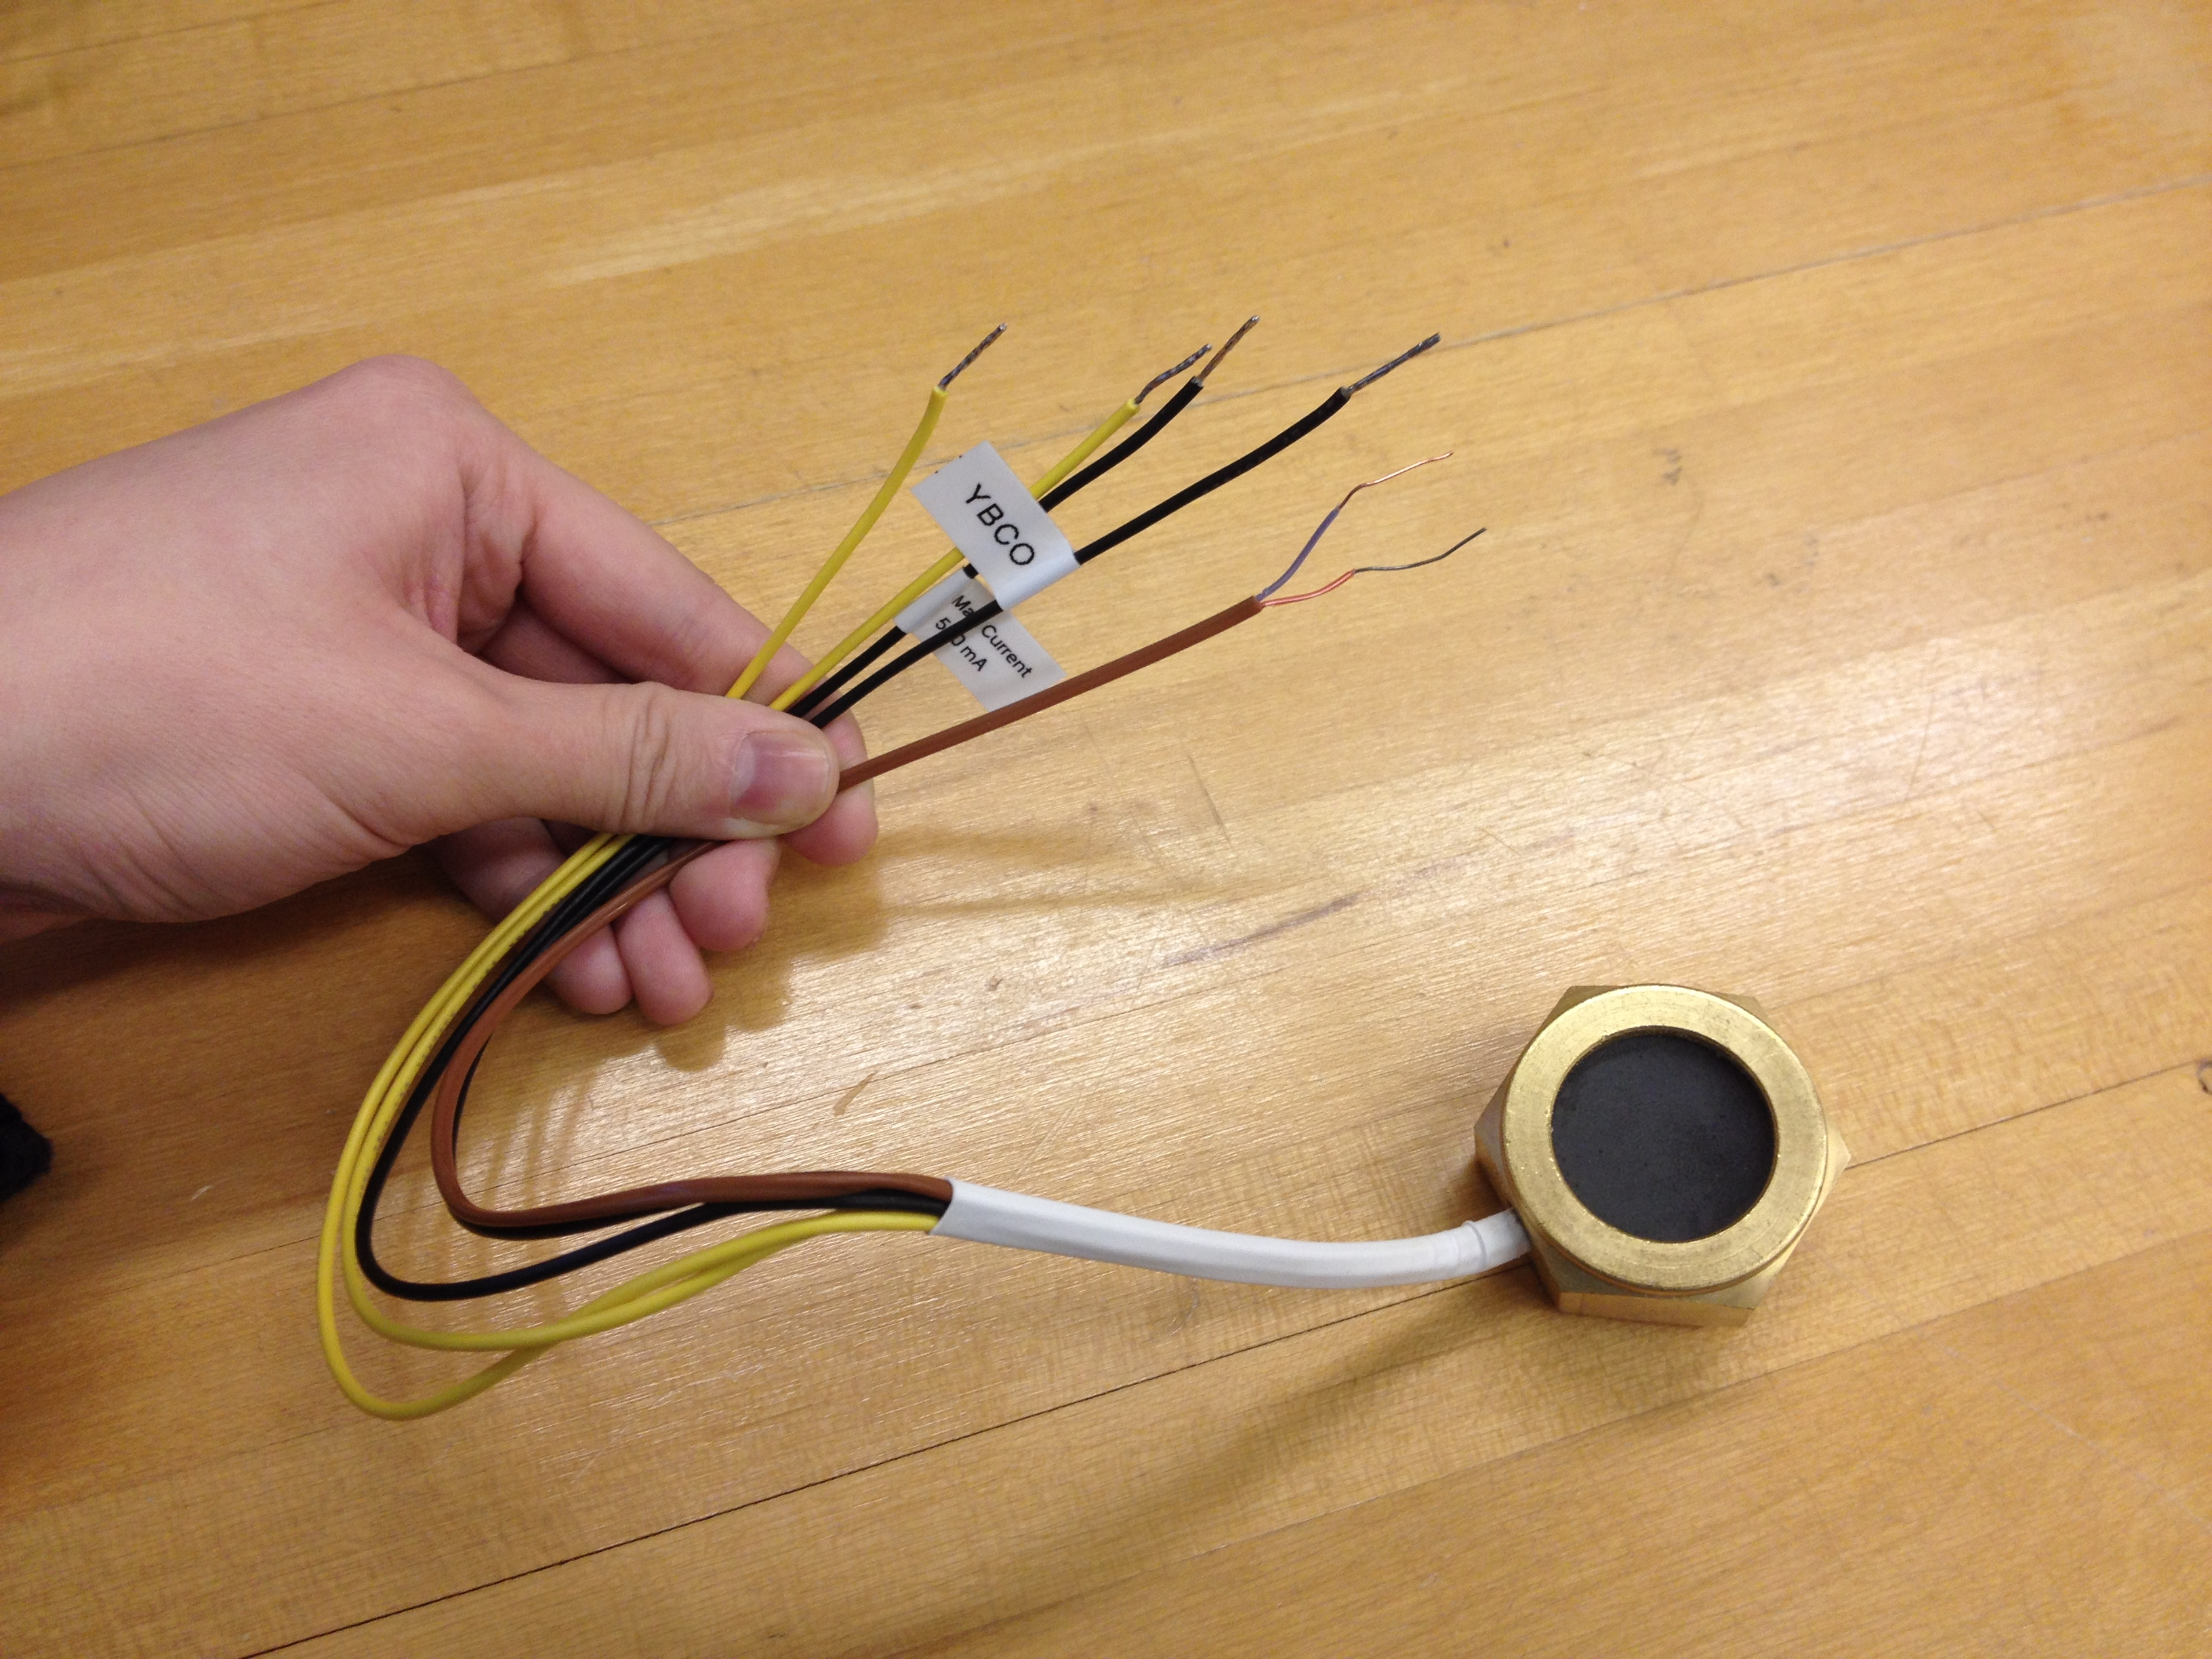
\includegraphics[width=14cm]{ybcosample.jpg}
\caption{Picture of the device, including YBCO sample (the black disk on top), thermocouple (brown lead), current (black leads) and voltage probes (yellow leads)}
\label{sample}
\end{figure}

When superconducting, the material has a very low resistance, which means the resistance of the leads of the probes becomes non-negligible. Therefore a method called four point probe is employed so that only the resistance of the material is measured, not that of the leads. The circuit is shown in Fig. \ref{fpp}. The black rectangle at the bottom represents the YBCO sample, an ammeter is connected in series with the sample through leads 1 and 4, and a voltmeter is connected in parallel with the sample through leads 2 and 3. Then the resistance of the sample could be calculated using Ohm's Law:

\begin{equation}
R=\frac{V}{I}
\label{ohm}
\end{equation}

where V and I are readings of the voltmeter and ammeter respectively. The key point here is that leads 2 and 3 have to be inside leads 1 and 4, in terms of position on the sample. Picture the meters as ideal meters plus lead resistance. The advantage of doing so is that the ammeter approximately measures the current through the sample, because the resistance of the voltmeter is so much bigger than that of the superconductor that the current through the voltmeter is very close to zero; and the voltmeter only measures the voltage across the sample. However, i f the position of the ammeter and voltmeter were switched, as the right circuit shown in Fig. \ref{fpp}, the voltmeter would measure the voltage across the lead resistance of the ammeter and the sample resistance connected in parallel. The total resistance of the two in parallel would differ from the sample resistance a lot because when superconducting, the resistance of the sample is comparable to the resistance of the lead. \\

\begin{figure}[h]
\centering
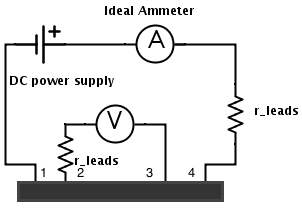
\includegraphics[width=8cm]{fourpointprobe2.png}
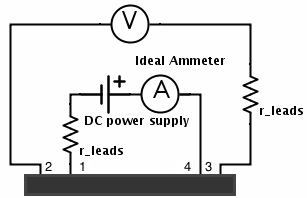
\includegraphics[width=8cm]{fourpointprobe3.png}
\caption{Schematic of four point probe. The right is the bad configuration. The circuits are drawn with online tool Scheme-it \cite{drawcircuit}.}
\label{fpp}
\end{figure}

The sample is connected to two digital multimeters (DMM) (top two in Fig. \ref{meters}) and one power source {bottom one in Fig. \ref{meters}}. The top one is measuring the voltage across the thermocouple, and the voltage can be translated into temperature according to the table in Fig. \ref{temp}. \\

\begin{figure}[h]
\centering
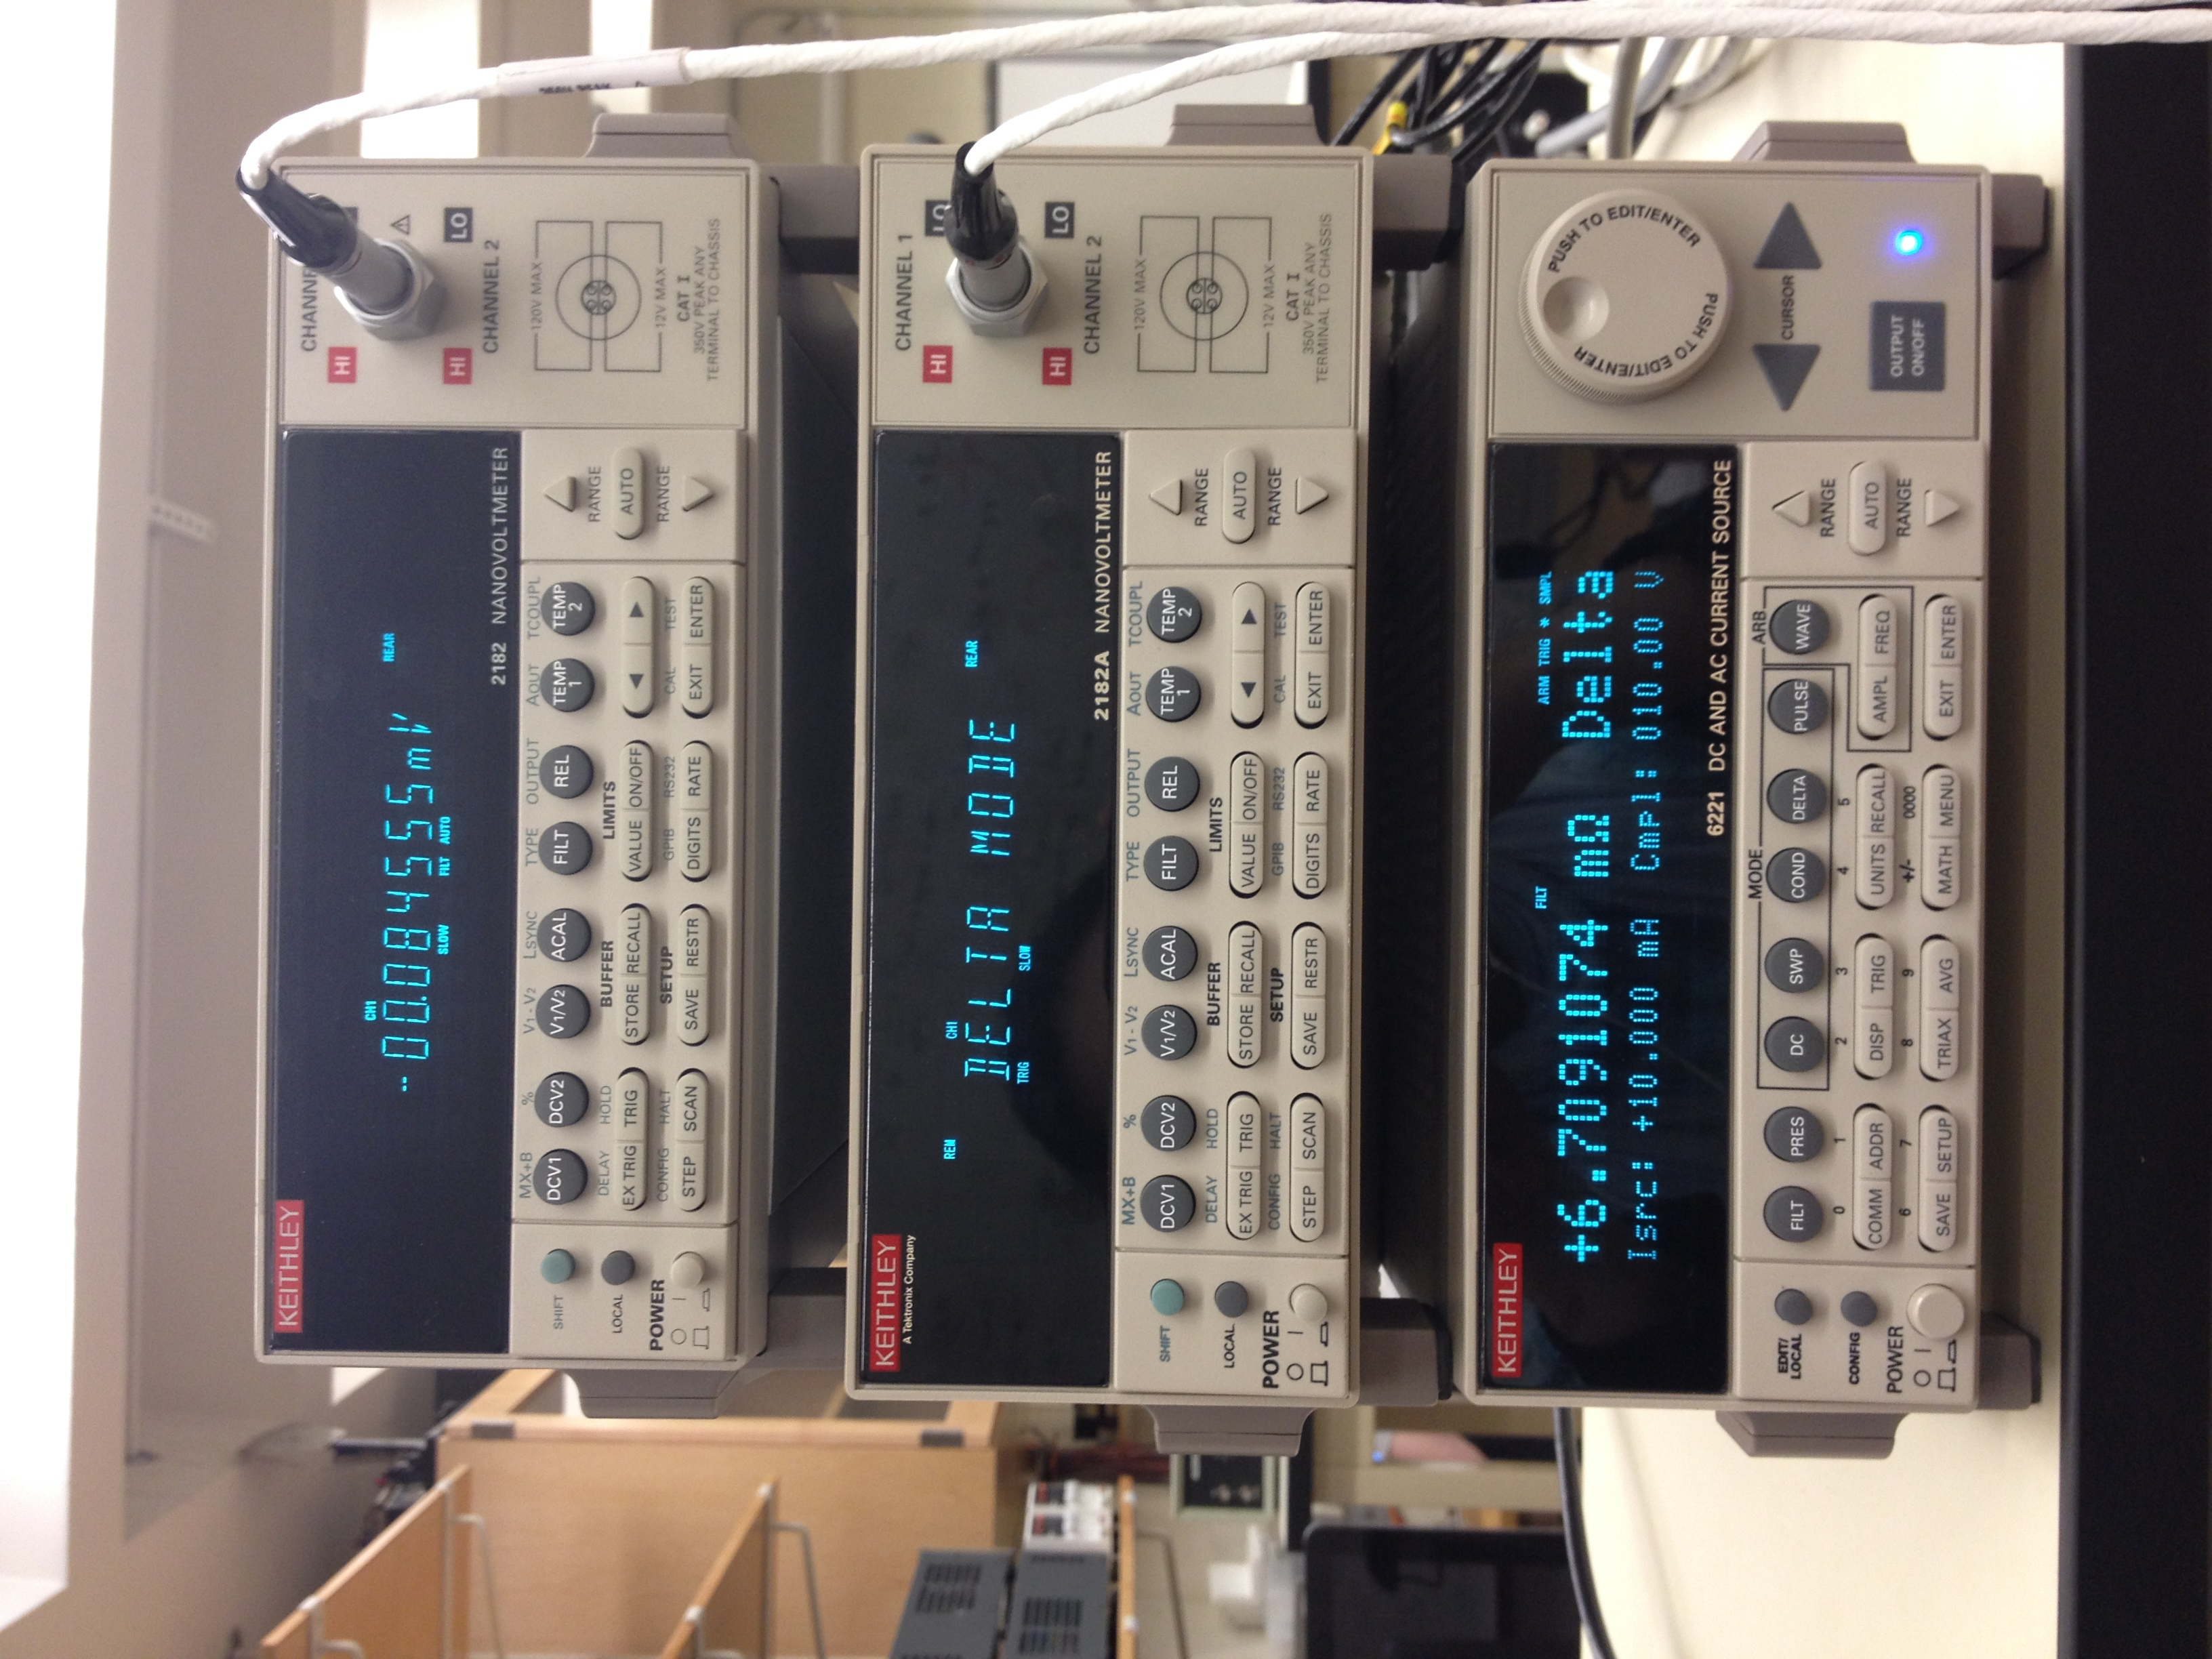
\includegraphics[width=10cm]{ybcometers.jpg}
\caption{The DMMs and power supply used. The top one measures the voltage of the thermocouple, the middle one measures the voltage across the sample, but the value is not shown on the screen under delta mode. And the bottom one is a power source that is in delta mode, and it reads the resistance of the YBCO sample.}
\label{meters}
\end{figure}

\begin{figure}[h]
\centering
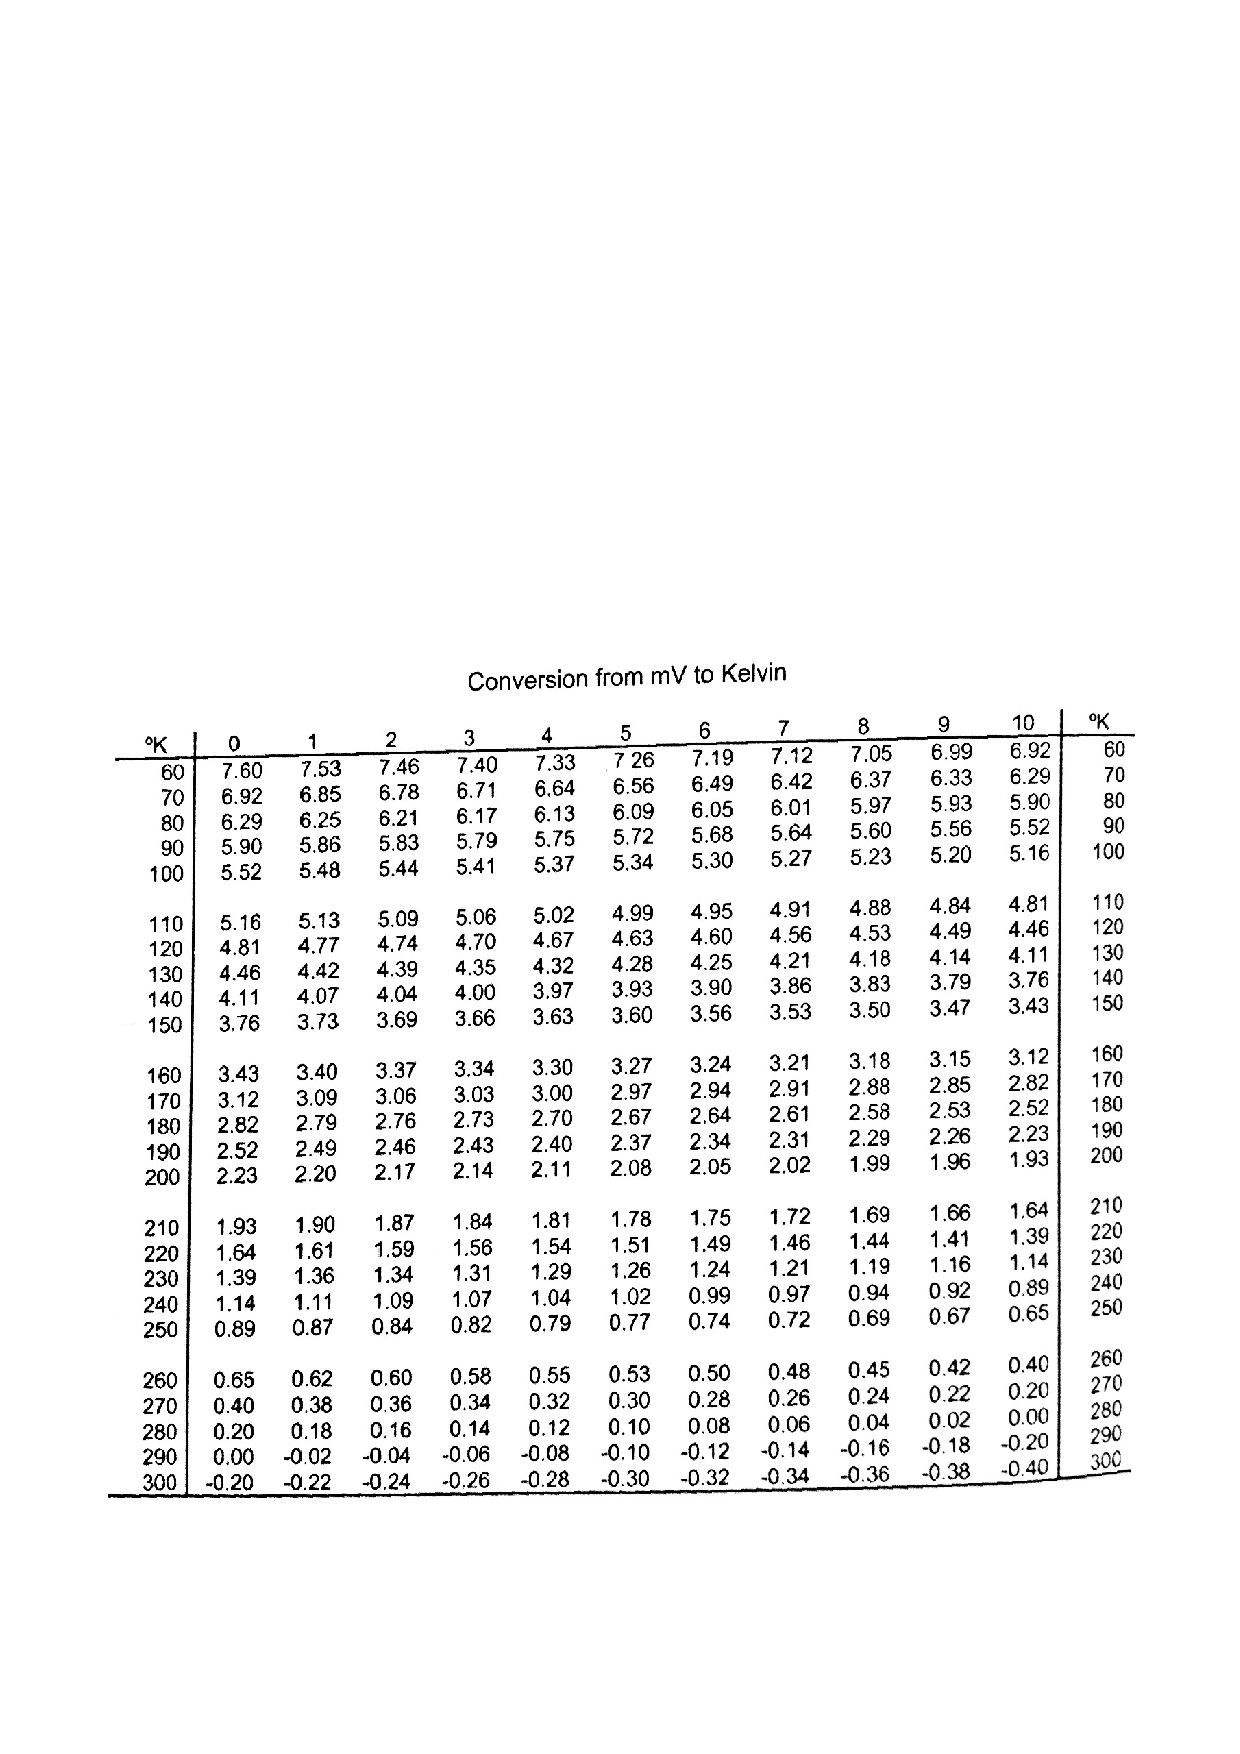
\includegraphics[width=14cm]{temperature.pdf}
\caption{The correlation between the temperature and the voltage across the thermocouple \cite{thermocouple}}
\label{temp}
\end{figure}

The source is the "DC power supply" in Fig. \ref{fpp} and Fig. \ref{fpp2}. Although it is labelled as DC power source, it is actually in delta mode, which means it is outputting a current alternating between positive and negative in the fashion of a square wave. The advantage of delta mode is that it can eliminate the affect of offsets measured by the voltmeter. When a positive current is passing through the sample, the voltmeter measures an offset and the real voltage signal across the sample, $V_{+}=V_{offset}+V_{signal}$; if the current is reversed, the voltage across the sample would also flip sign, but the offset would remain the same, $V_{-}=V_{offset}-V_{signal}$. From $V_{+}$ and $V_{-}$, the voltage due to the sample can be calculated. The middle DMM reads the two voltages and calculates $V_{signal}$ automatically. The middle DMM is also connected to the power supply at the back. The power source reads $V_{signal}$ from the middle DMM and then divides it by the current to get the resistance of the superconductor, which is shown on the screen in unit of m$\Omega$. By observing the temperature dependence of the resistance, the critical temperature of the superconductor could be found out. \\

However, the drawback of this setup is that we could not make computer record the data. So we videotaped the DMMs while the sample was cooled down by liquid nitrogen, and then transcribed the thermocouple voltage and superconductor resistance into analysis tool, i.e. Igor Pro, by hand. To test the current dependence of the critical temperature of the material, four sets of data are collected, with current output of the power supply being 0.1mA, 1mA, 10mA and 100mA respectively.\\

\subsection{BSCCO}

The setup of the experiment on BSCCO is shown in Fig. \ref{bsccosetup}. The device is also put in a plastic-foam cup and covered by sands. This device is designed in the same manner as the YBCO sample using four point probe.

\begin{figure}[h]
\centering
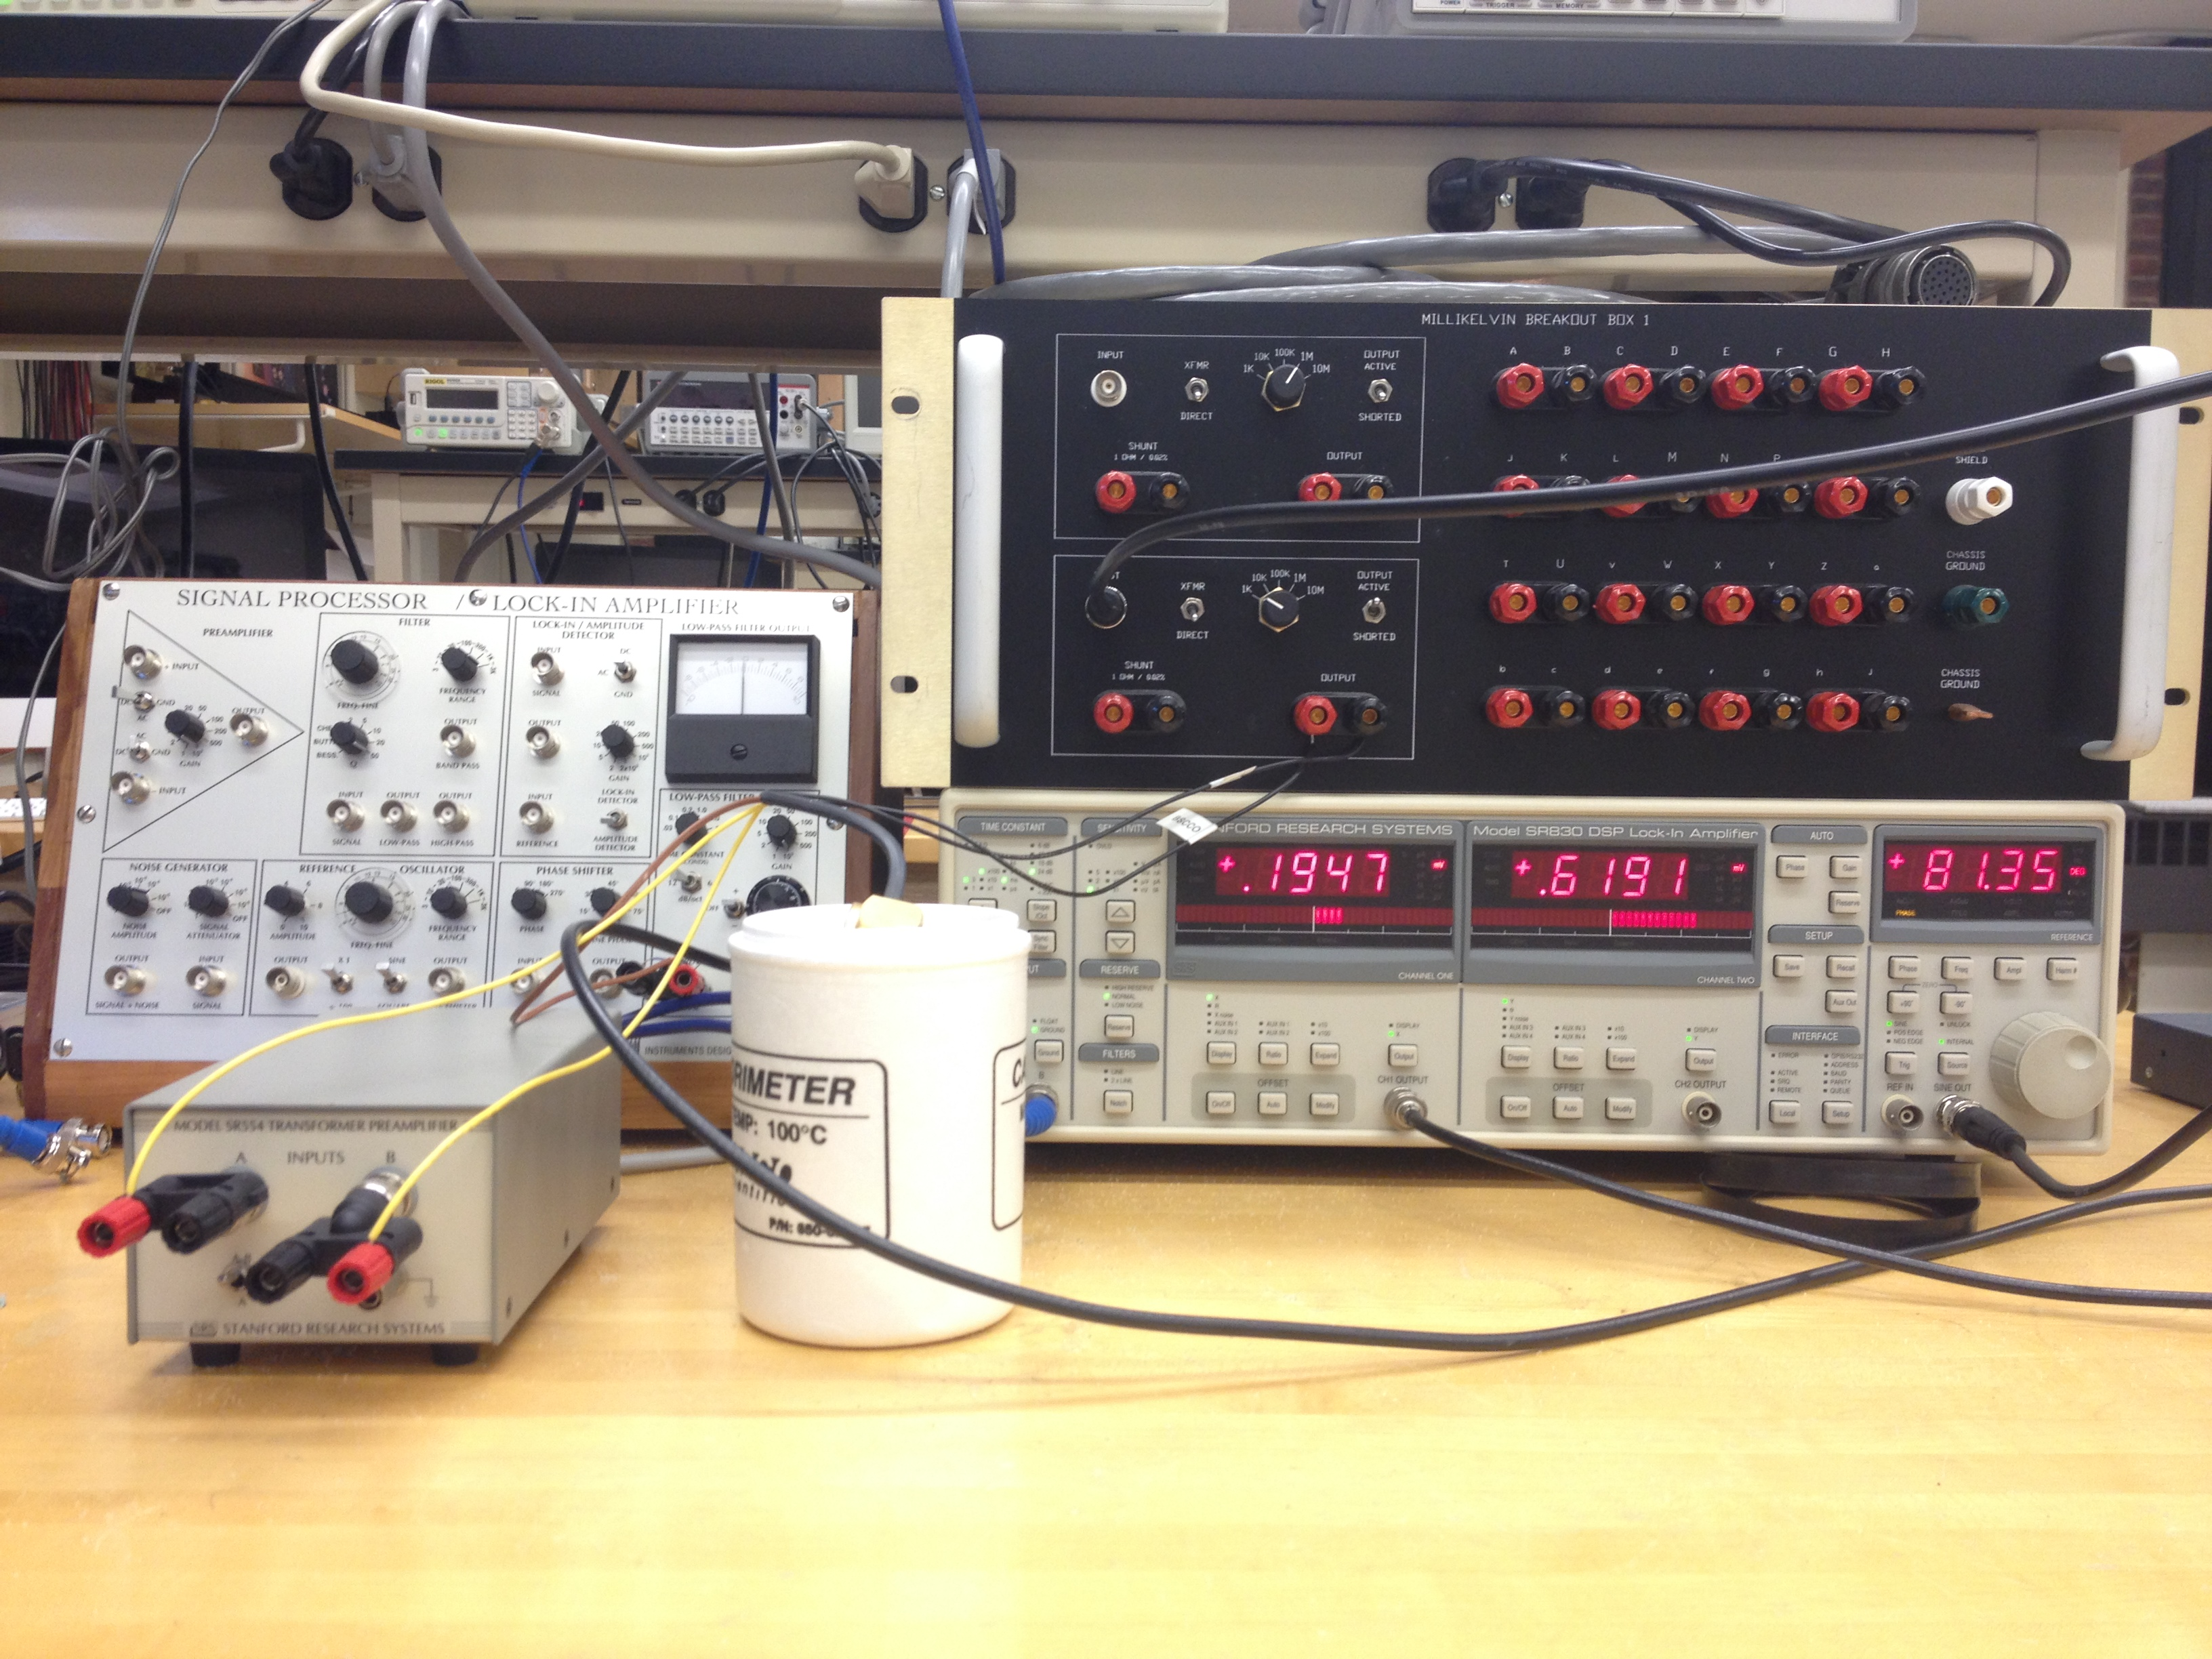
\includegraphics[width=14cm]{bsccosetup.jpg}
\caption{The setup of experiment of BSCCO.}
\label{bsccosetup}
\end{figure}

The thermal couple is connected to the left lock-in amplifier in Fig. \ref{bsccosetup}, which has a time constant of 1s and a gain of 1000. The output is fed to a DMM which is read by the computer. \\

A Model SR830 DSP lock-in amplifier (simplified as SR830 lock-in amplifier, gray equipment on the lower right in Fig. \ref{bsccosetup}) is employed in this experiment. The most important feature of this lock-in amplifier is that it feeds the sample a sine signal and then it detects the in-phase and out-of-phase feedbacks from the sample separately, with in-phase feedback shown in channel 1 (left) and the out-of-phase one shown in channel 2 (right). \\

When wires are close together, they form a capacitor. When they curl, they become inductors. In both situations the wires bring in noise if we only want to know the voltage across the resistor. Normally the noise would be so small that it could be safely neglected. However, the resistance of the superconductor drops to such a low level that that noise becomes dominant. To distinguish between signal and noise, a sine input is introduced. The resistor outputs a voltage that is in-phase with the input, while the "capacitors" and "inductors" formed by wires yield voltage that has a $\pi/2$ phase delay. We could filter out the noise by only taking the in-phase voltage. \\

SR830 lock-in amplifier has a sine voltage output, whose peak to peak value is measured to be $2.80 \pm 0.02 V$. Therefore it has the root mean square value is $0.990\pm0.007V$. This output is fed to the input of a breakout box (the black box in the upper right in Fig. \ref{bsccosetup}), and then converted to a current through a resistor of $1k\Omega$. This current now acts as the "DC power supply" in Fig. \ref{fpp}, and is introduced into the circuit through the black wires (the current probe). The yellow leads (the voltage probe) are connected to a transformer preamplifier with a gain of 500, which is then connected back to the SR830 lock-in amplifier. The in-phase channel (CH1) is read by another DMM which ultimately communicates with the computer. LabView is used to collect the readings from the two DMMs: the voltage from the thermal couple and the in-phase voltage signal from the SR830 lock-in amplifier. \\

The resistance of the superconductor can be calculated by

\begin{equation}
R_{superconductor} = \frac{V_{in-phse}/g}{I}
\label{rofs}
\end{equation}

where

\begin{equation}
I=\frac{V_{rms}}{R_{breakout}}
\label{current}
\end{equation}

and $V_{in-phse}$ is the in-phase voltage measured, $g=500$ is the gain of the transformer, $V_{rms}=0.990\pm0.007V$ is the maximal input sine voltage from SR830 lock-in amplifier and $R_{breakout}=1k\Omega$ is the resistance in the breakout box. And the temperature of the sample could be converted from the voltage across the thermal couple using the table in Fig. \ref{temp}.\\


%____________Results____________________________________________
\section{Results}

\subsection{YBCO}
The temperature, converted from thermal couple voltage and resistance of the superconductor are collected and plotted, as shown in Fig, \ref{ybco10ma}. Then the high temperature part, the transit part and the low temperature are fitted with lines. The intersections of the high temperature and the transit part, and of the low temperature and the transit part are found. The critical temperature is then calculated by averaging the temperatures of the two intersecting points. Fig. \ref{ybcoanalysis} shows the analysis. (Figures of analyses of other data sets are shown in the appendix.)

\begin{figure}[h]
\centering
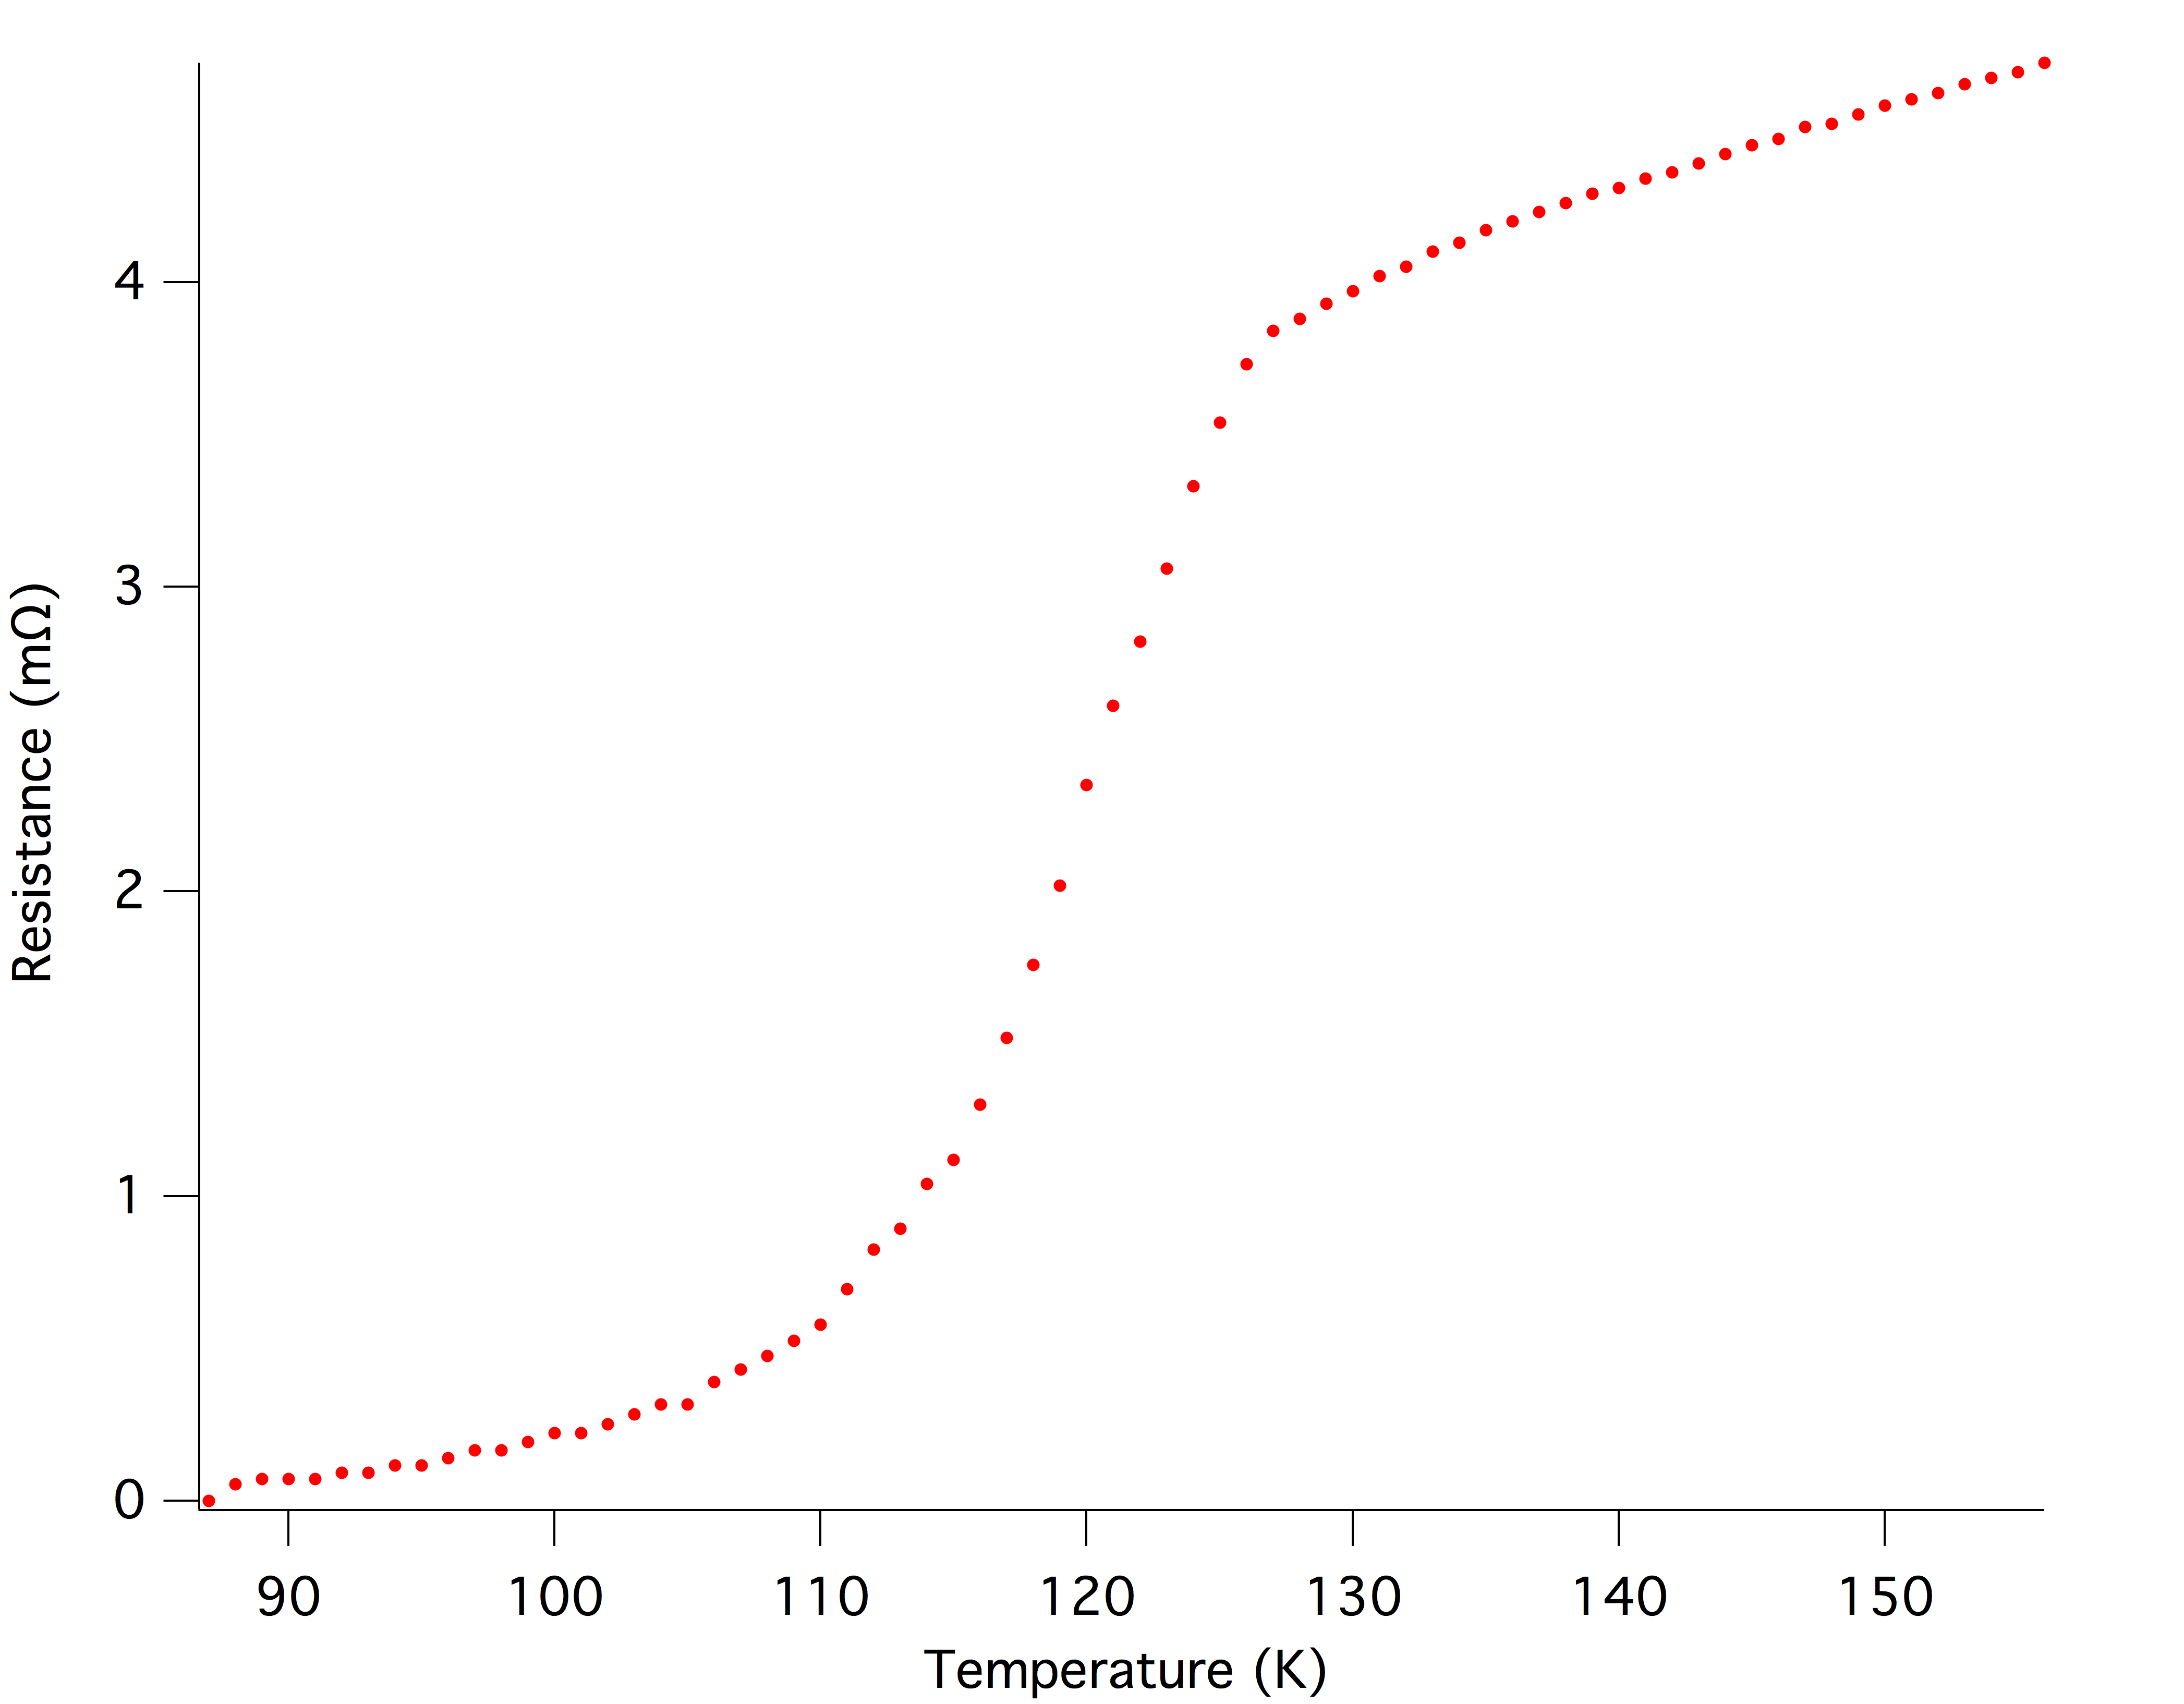
\includegraphics[width=14cm]{ybco10ma_raw.png}
\caption{Resistance vs. temperature of YBCO when current is 10mA}
\label{ybco10ma}
\end{figure}

\begin{figure}[h]
\centering
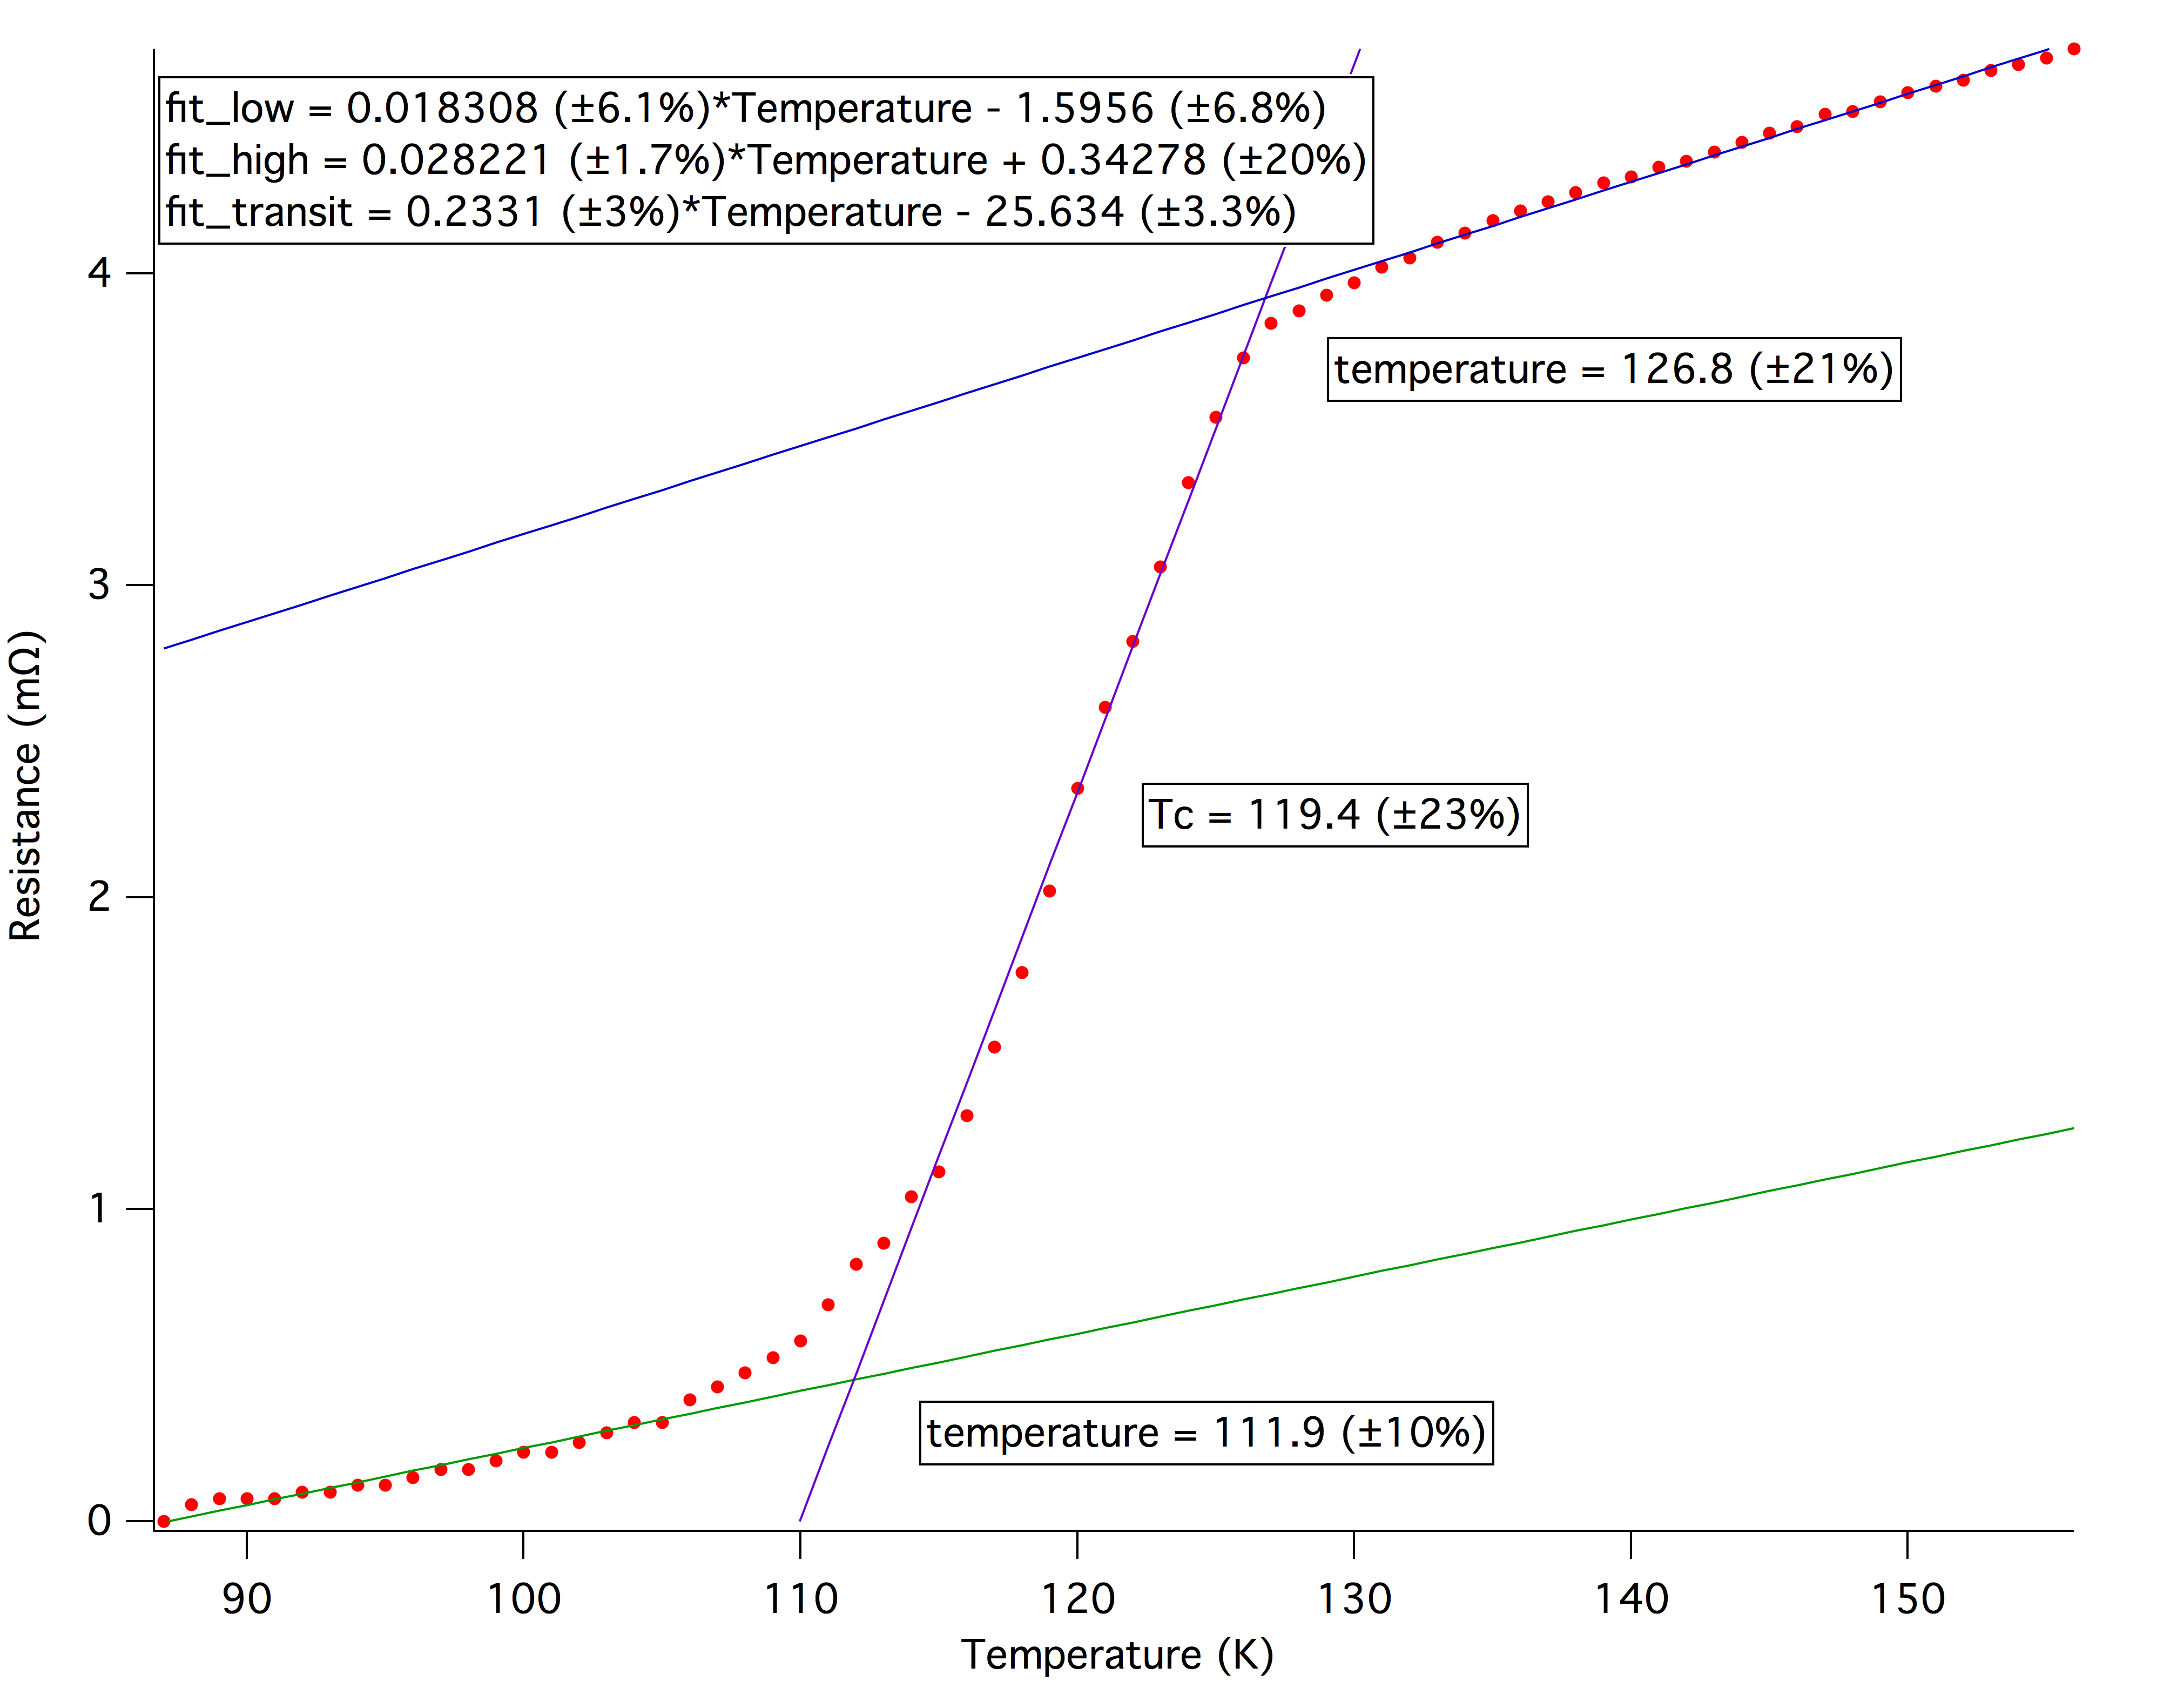
\includegraphics[width=14cm]{ybco10ma.png}
\caption{Analysis of data. The percentage uncertainties are indicated in the parenthesis. }
\label{ybcoanalysis}
\end{figure}

The critical temperatures of YBCO at different currents are found and listed in Table. \ref{ybcodata}. The critical temperature in the last row are calculated from data collected by using the BSCCO setup for comparison. \\

It can be seen that the uncertainties for the critical temperatures are huge, which is a result of the small number of data points we have. And that is because we have to transcribe the data from videos into computers by hand, which is not a very efficient or economical method.\\

\begin{table}[h]
\centering
\caption{YBCO Critical Temperature}
\begin{ruledtabular}
\begin{tabular}{ c c c}
Current & Critical Temperature & Uncertainty\\
(mA) & (K) & (\%)\\
\hline
0.1 & 115.9 & 60 \\
1 & 117.6 & 73 \\
10 & 119.4 & 23 \\
100 & 115.5 & 53 \\
N/A & 109.5 & 3.8 \\
\end{tabular}
\end{ruledtabular}
\label{ybcodata}
\end{table}

\subsection{BSCCO}
Only one set of data is obtained for BSCCO. The raw data is shown in Fig. \ref{bsccoraw}. The same line-fitting is done to the BSCCO data. However, the data of BSCCO are not as clean as that of YBCO: the high temperature part (low thermal couple voltage part) does not show an obvious linear relation. Therefore only the first linear section before the transit part is fitted (thermal couple voltage ranges from around 3.5V to 4.5V). The analysis is shown in Fig. \ref{bsccoanalysis}. The critical temperature is found to be $116\pm6$K.\\

\begin{figure}[h]
\centering
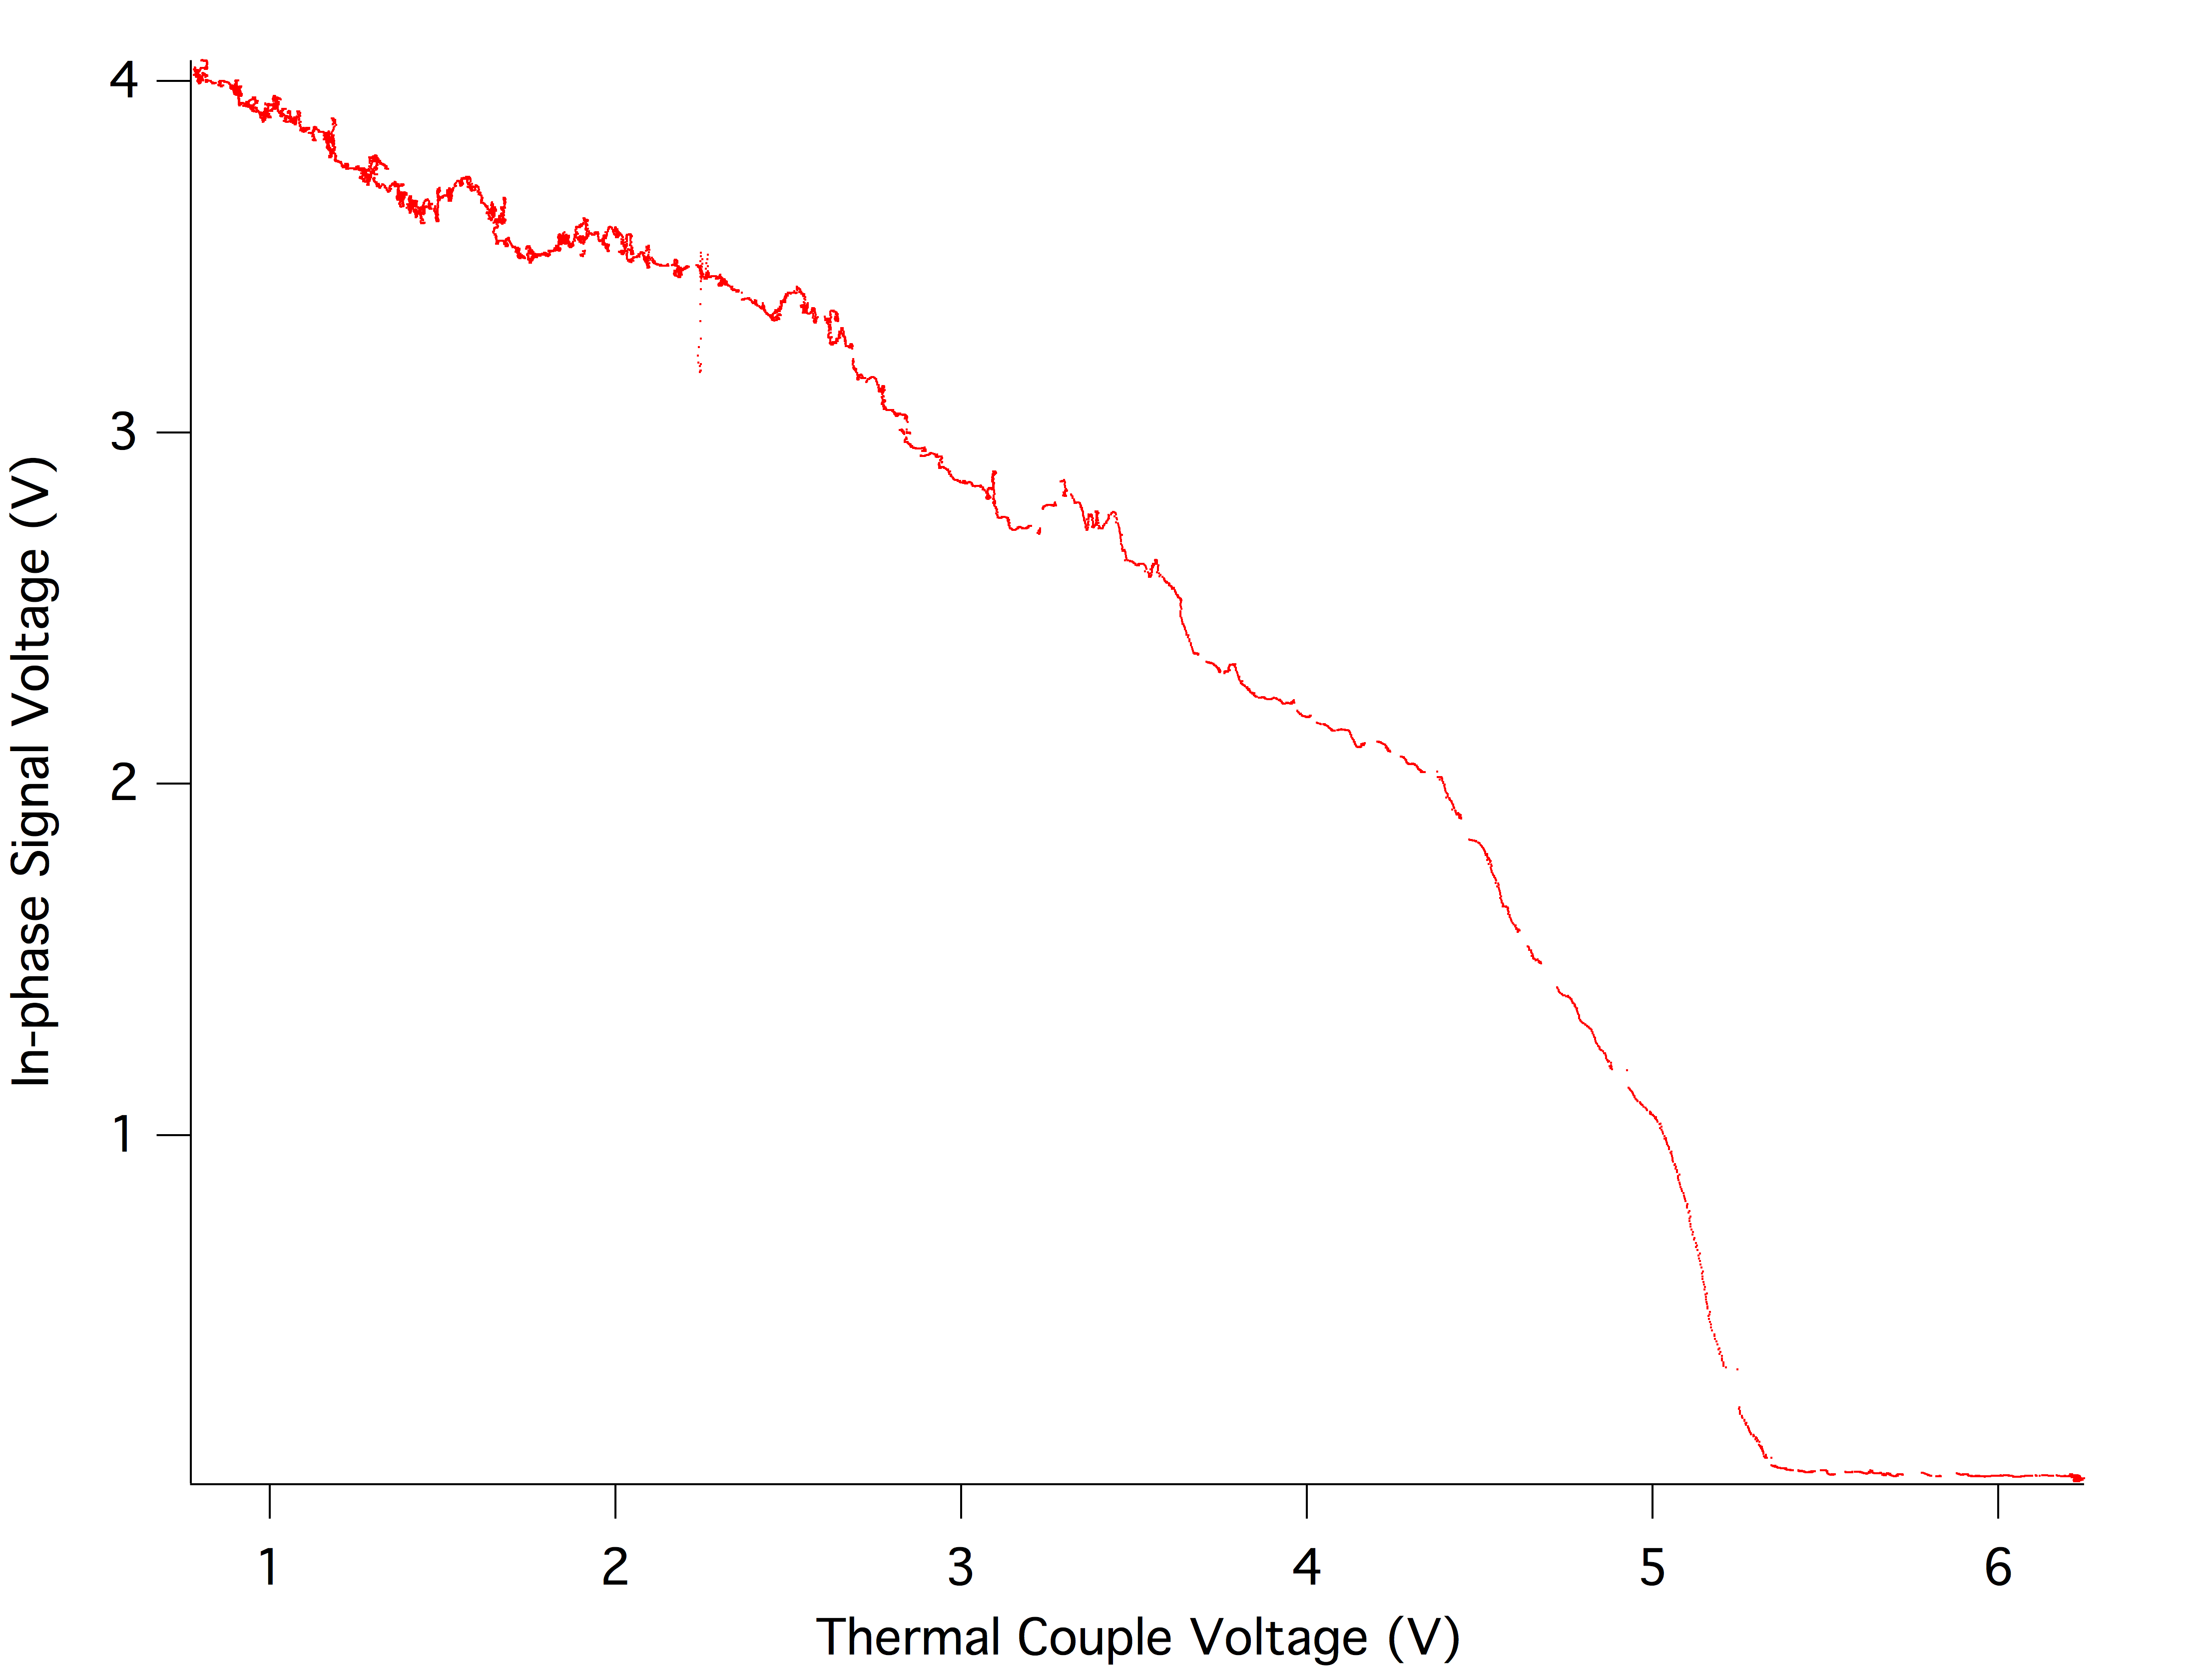
\includegraphics[width=14cm]{bscco_heating_raw.png}
\caption{Raw data of BSCCO. The x axis is the thermal couple voltage, which can be converted to temperature. The y axis is the in-phase signal voltage, which can be converted to resistance using Eq. \ref{rofs}.}
\label{bsccoraw}
\end{figure}

\begin{figure}[h]
\centering
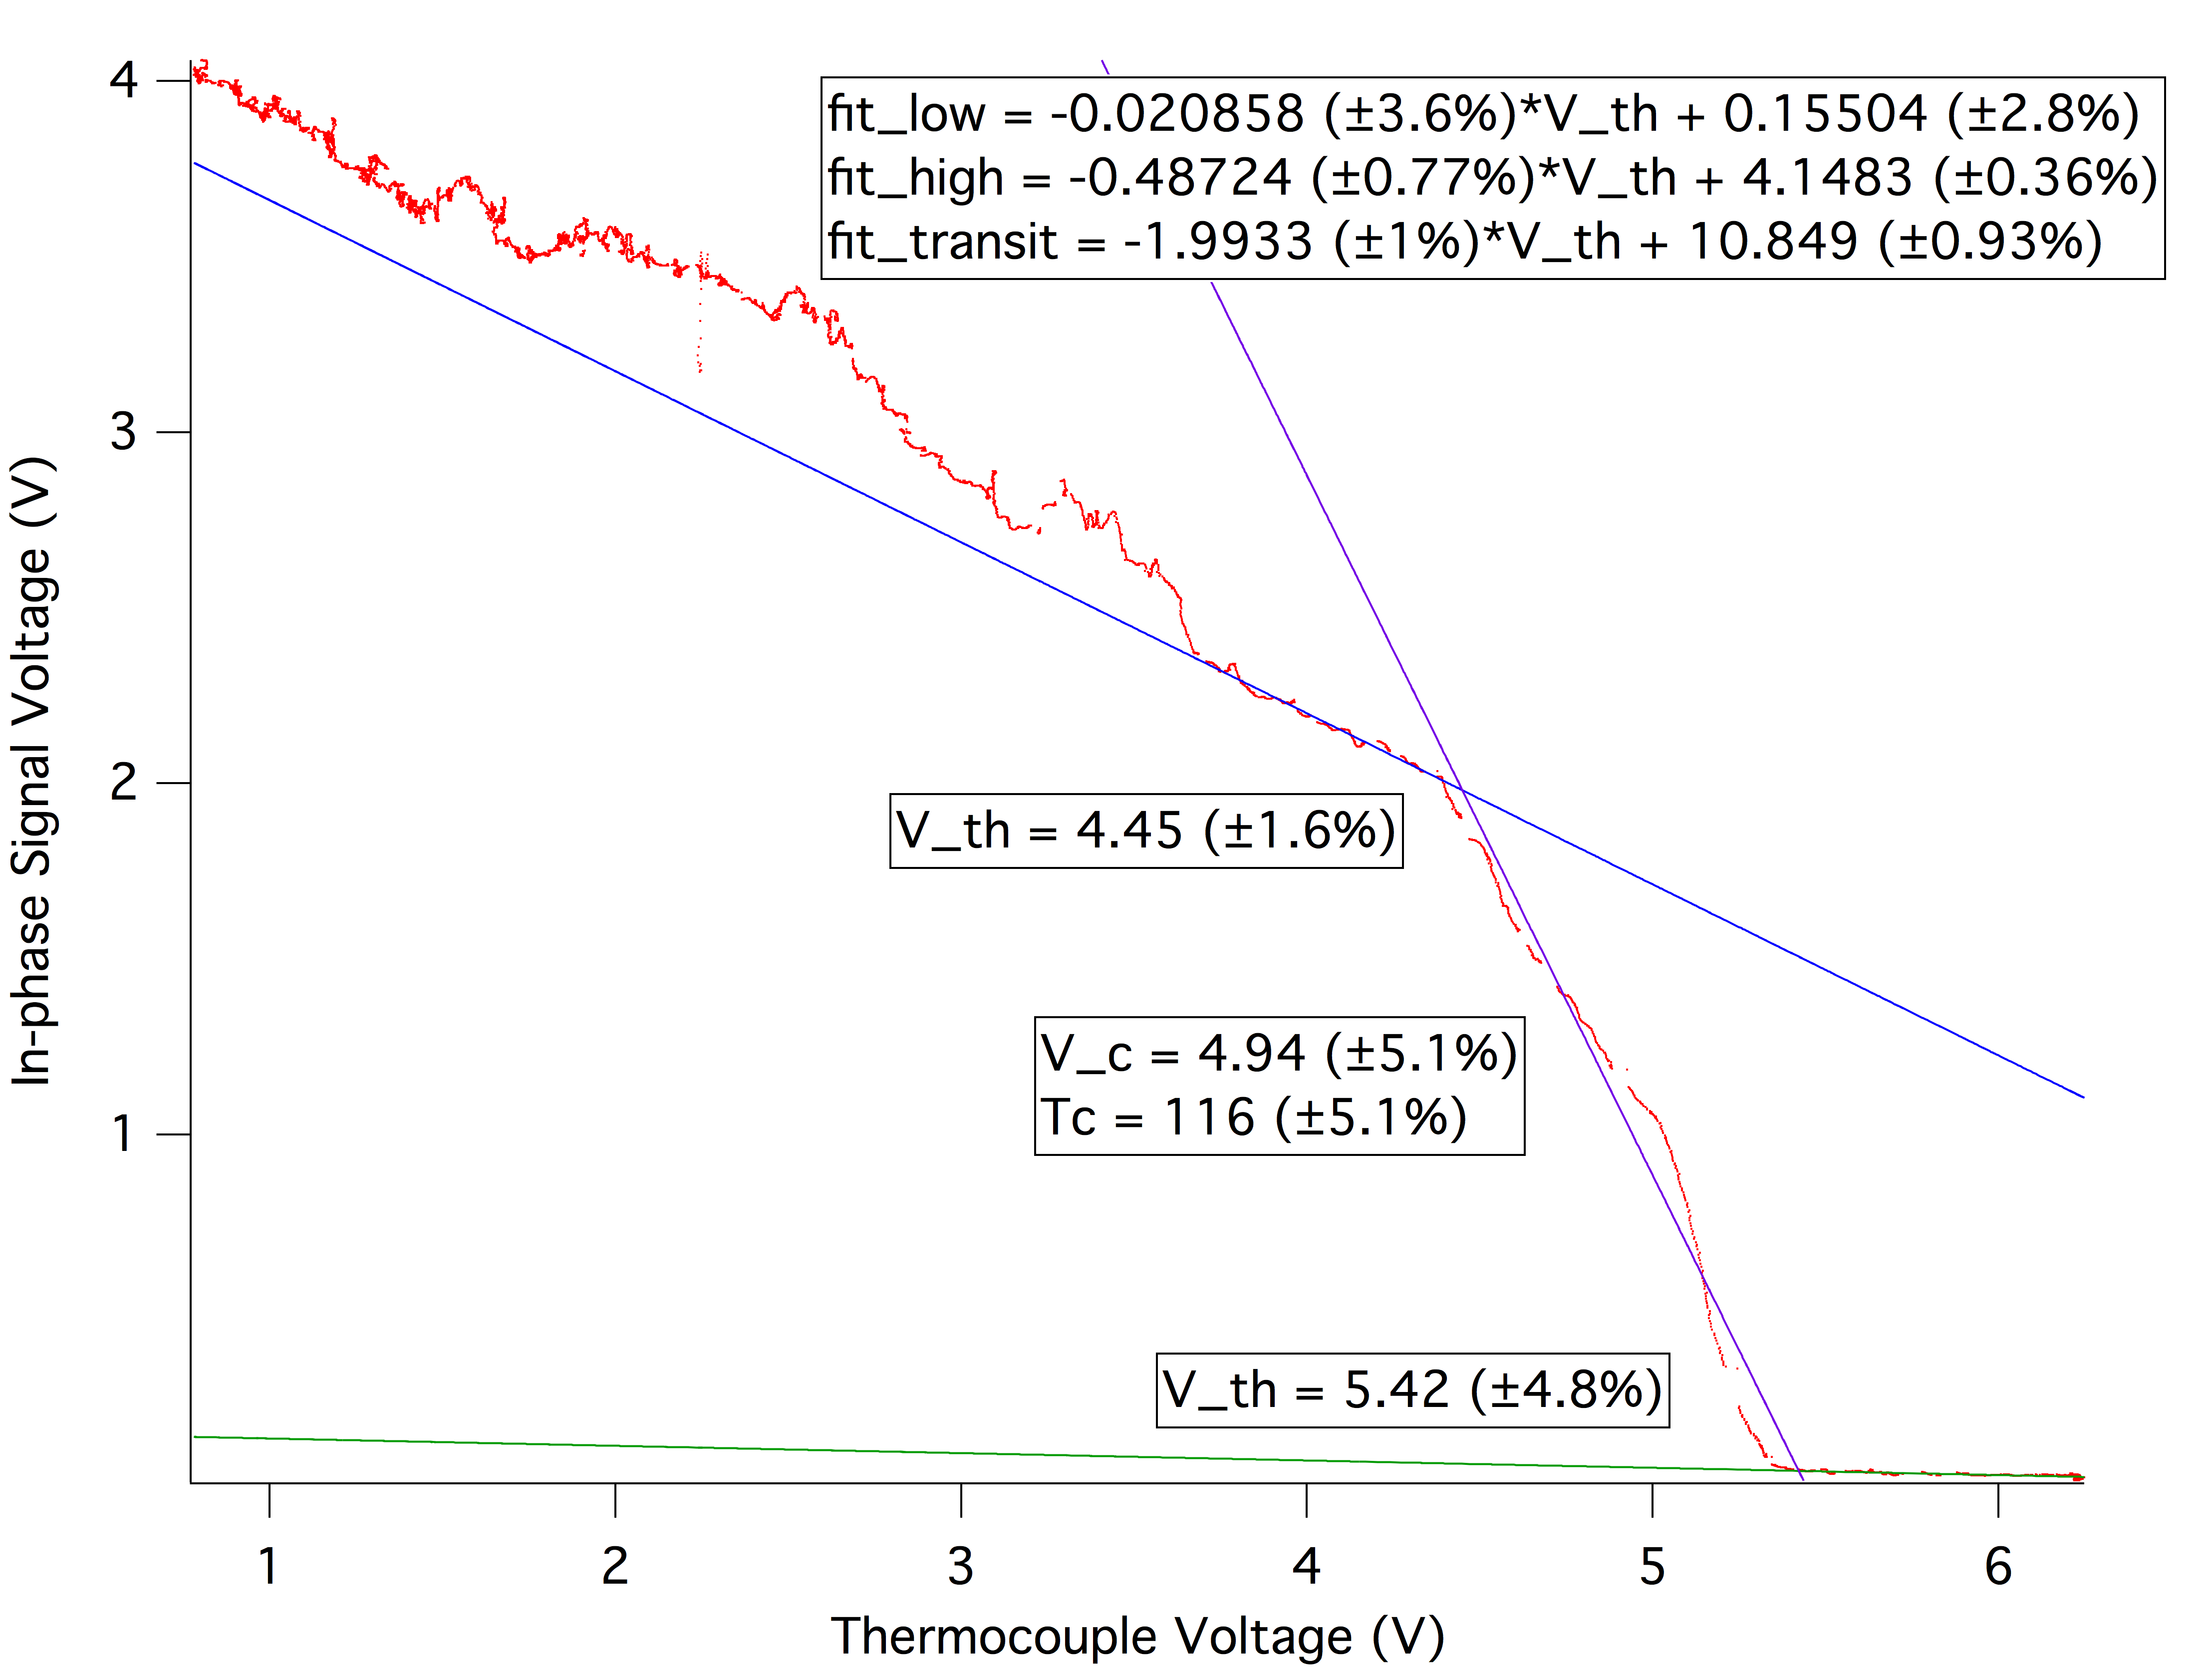
\includegraphics[width=14cm]{bscco_heating.png}
\caption{Analysis of BSCCO data}
\label{bsccoraw}
\end{figure}



%____________Discussion____________________________________________
\section{Discussion}

For both samples we were able to observe the transition into the superconducting phase. For the YBCO sample, we see the critical temperature varies across different current settings, but no reliable correlation is found from our data. To find the temperature at a certain resistance value, we need to look at the calibration data of the thermocouple, which have a temperature increment of 1K. This sets the resolution of the data we have, imposing a limit as to how well we can resolve the resistance's dependence on temperature. One potential solution for this is to input all the data points of the thermocouple calibration into computer then find a fit to them, allowing us to better resolve the intermediate temperatures between integer values. In addition, due to the limitation of manual data collection, we were not able to cover the full temperature range of interest, introducing larger errors in the linear region fittings.\\

The critical temperature for the YBCO sample ranges from 109.5K to 119.4K across different current values, inconsistent with our expectation based on the commonly accepted value of 92K. Since all the results are much higher than the expected value, we suspect that the thermocouple used in this experiment introduced an offset. The calibration data we used and the actual behaviors of the thermocouple may mismatch-- the thermocouple produces a lower voltage than documented, making the measured temperature at any point higher than the actual temperature. We do not have a temperature reference to verify the calibration data of the thermocouple, so we cannot be sure whether this is the origin of the offset. \\

For the BSCCO sample, we could not see clear linear region above the final transition area. This could be due to the existence of the multiple superconductive transitions of BSCCO-- the sample begins to transition into its first superconducting at the first transition temperature, then the second, and the third. The three phase transitions may overlap with each other, imposing a difficulty to fit to the linear region. In addition, due to the roughness of the data we were not able to determine the individual transition temperatures. \\



%____________Conclusion____________________________________________
\section{Conclusion}

The critical temperatures we found for YBCO at 0.1, 1, 10, and 100mA are 115.9K, 117.6K, 119.4K, and 115.5K, respectively. We were not able to determine the critical temperature's dependence on current due to a lack of data points. In addition, with our data for thermocouple calibration, we could not better resolve the temperature since we only knew the thermocouple voltage data for each integer Kelvin. If we have a function describing the thermocouple voltage's dependence on temperature, we could have critical temperature values that are more precise. We would then also need a LabVIEW virtual instrument that can record data from the instruments employed in this experiments simultaneously to record data more efficiently.\\

The commonly accepted value for YBCO critical temperature from previous experiments is 92K, significantly different from our final results. To make our value more precise, we would either need another thermocouple that is well calibrated to our data, or work with our current thermocouple and perform calibration on it using some temperature reference.\\

Our final value for BSCCO critical temperature is $116\pm6$K. This result agrees with the expected value of 110K within uncertainty. \\

As we observed, the YBCO and BSCCO samples exhibit superconducting phenomenon at sufficiently low temperatures.\\


\begin{acknowledgments}

We gratefully acknowledge Nathanael Fortune and Dana Parsons, who helped with the experimentation and editing of this experiment. This work was supported by the Smith College Physics Department.

\end{acknowledgments}


\begin{thebibliography}{99}

%\bibitem{wik} Double Slit Experiment, \url{<http://upload.wikimedia.org/wikipedia/commons/c/c2/Single_slit_and_double_slit2.jpg/>}.
\bibitem{drawcircuit} Scheme-it, \url{http://www.digikey.com/schemeit}
\bibitem{thermocouple} Experiment Guide For Superconductor Demonstrations, p.12

\end{thebibliography}

%\newpage   % Start a new page for tables

%____________Appendix_____________________________________________
\clearpage
\begin{appendix}
\section{Figures of analyses}

\begin{figure}[h]
\centering
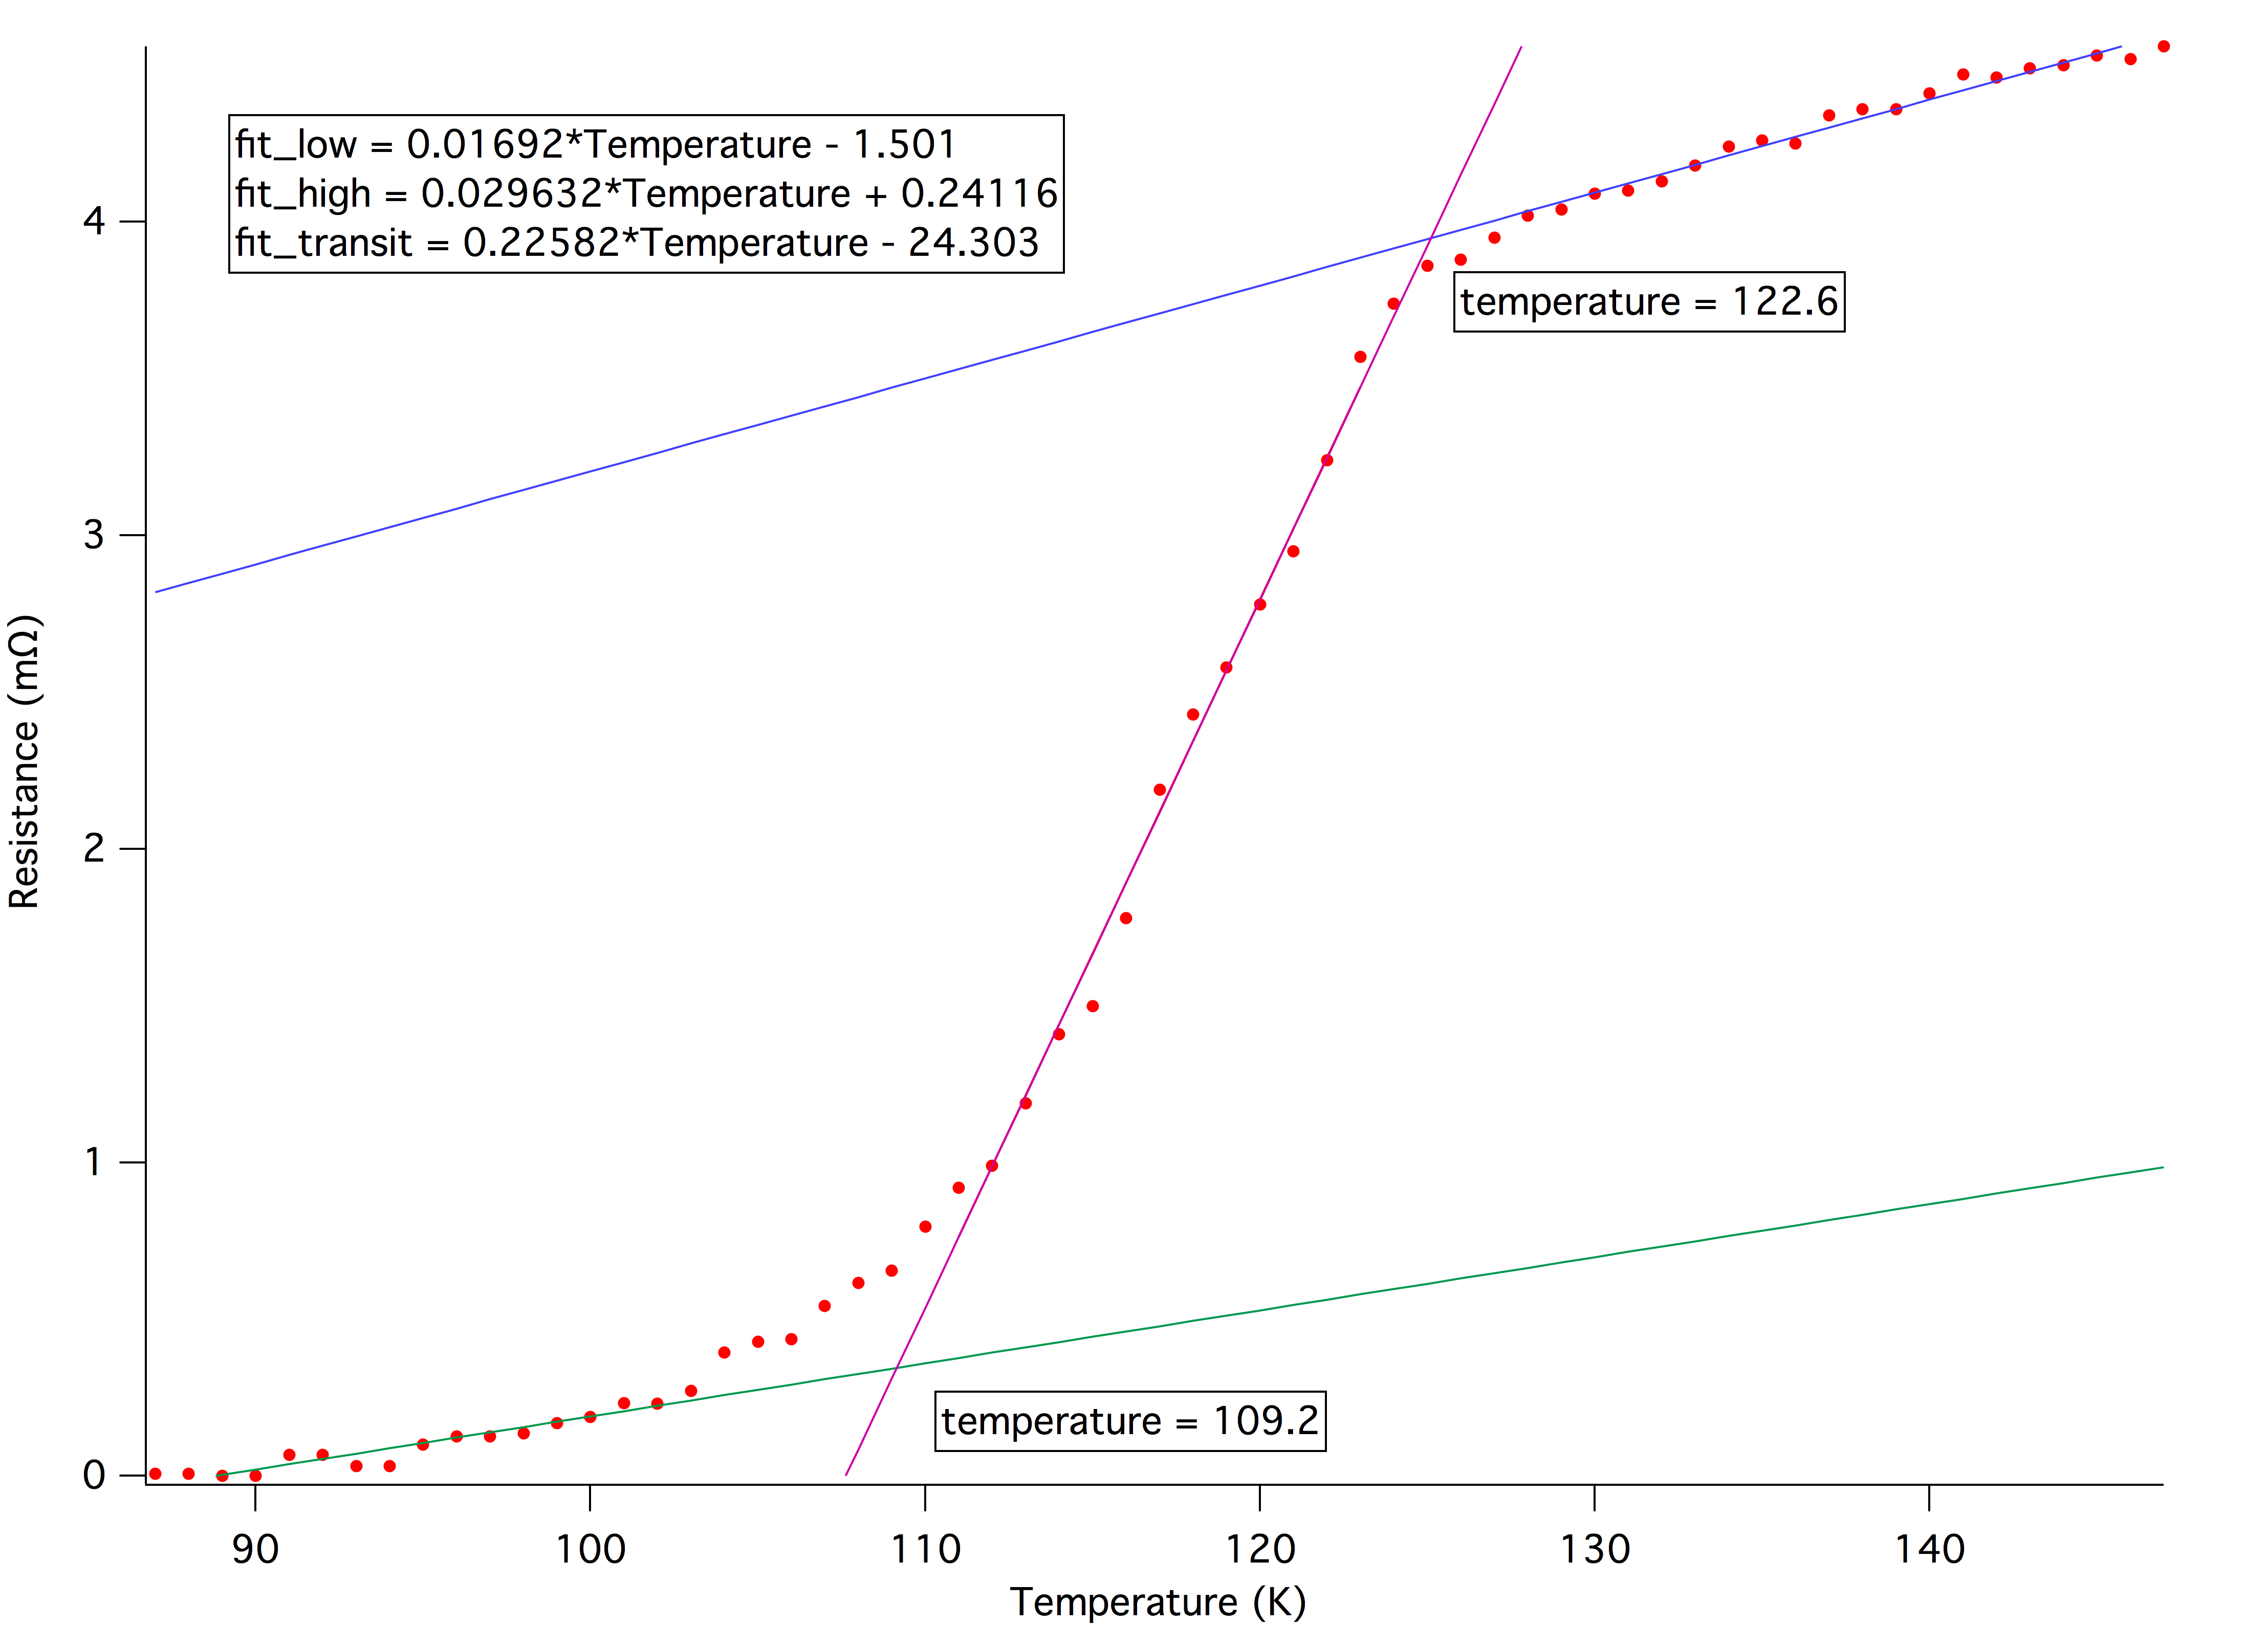
\includegraphics[width=11cm]{ybco01ma.png}
\caption{Analysis of data at current equal to 0.1mA }
\label{ybcoanalysis2}
\end{figure}

\begin{figure}[h]
\centering
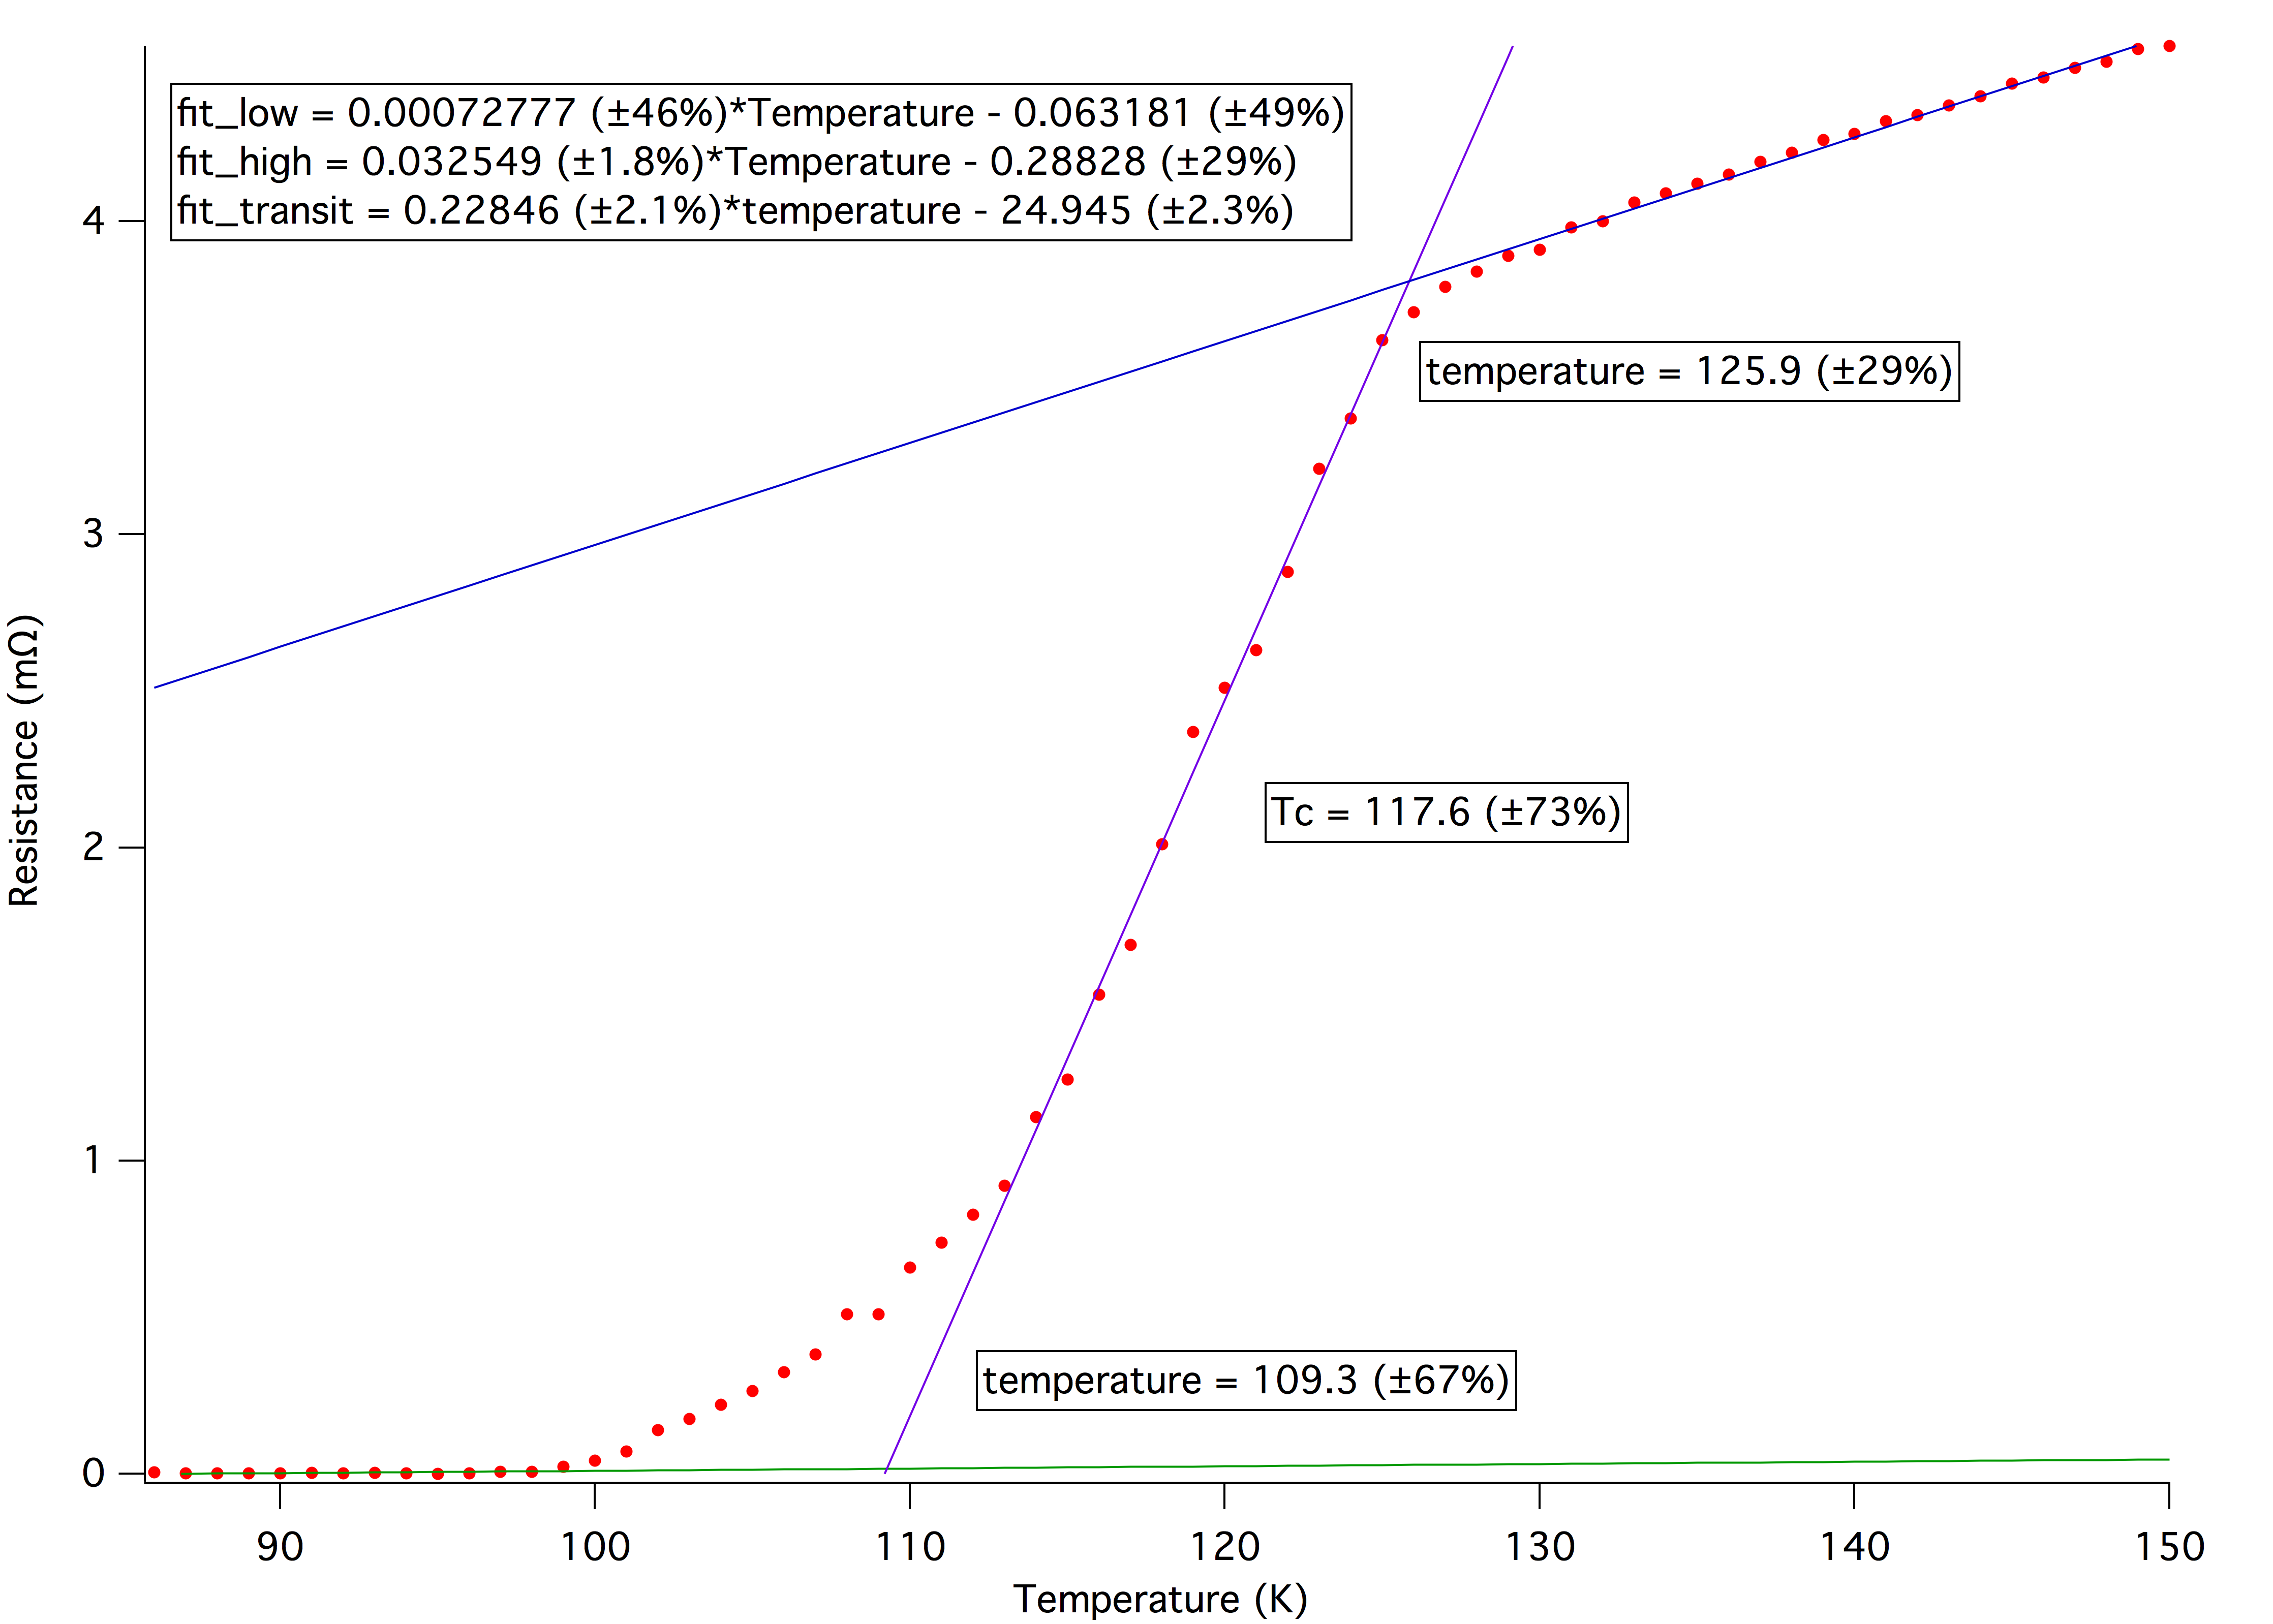
\includegraphics[width=11cm]{ybco1ma.png}
\caption{Analysis of data at current equal to 1mA }
\label{ybcoanalysis3}
\end{figure}

\begin{figure}[h]
\centering
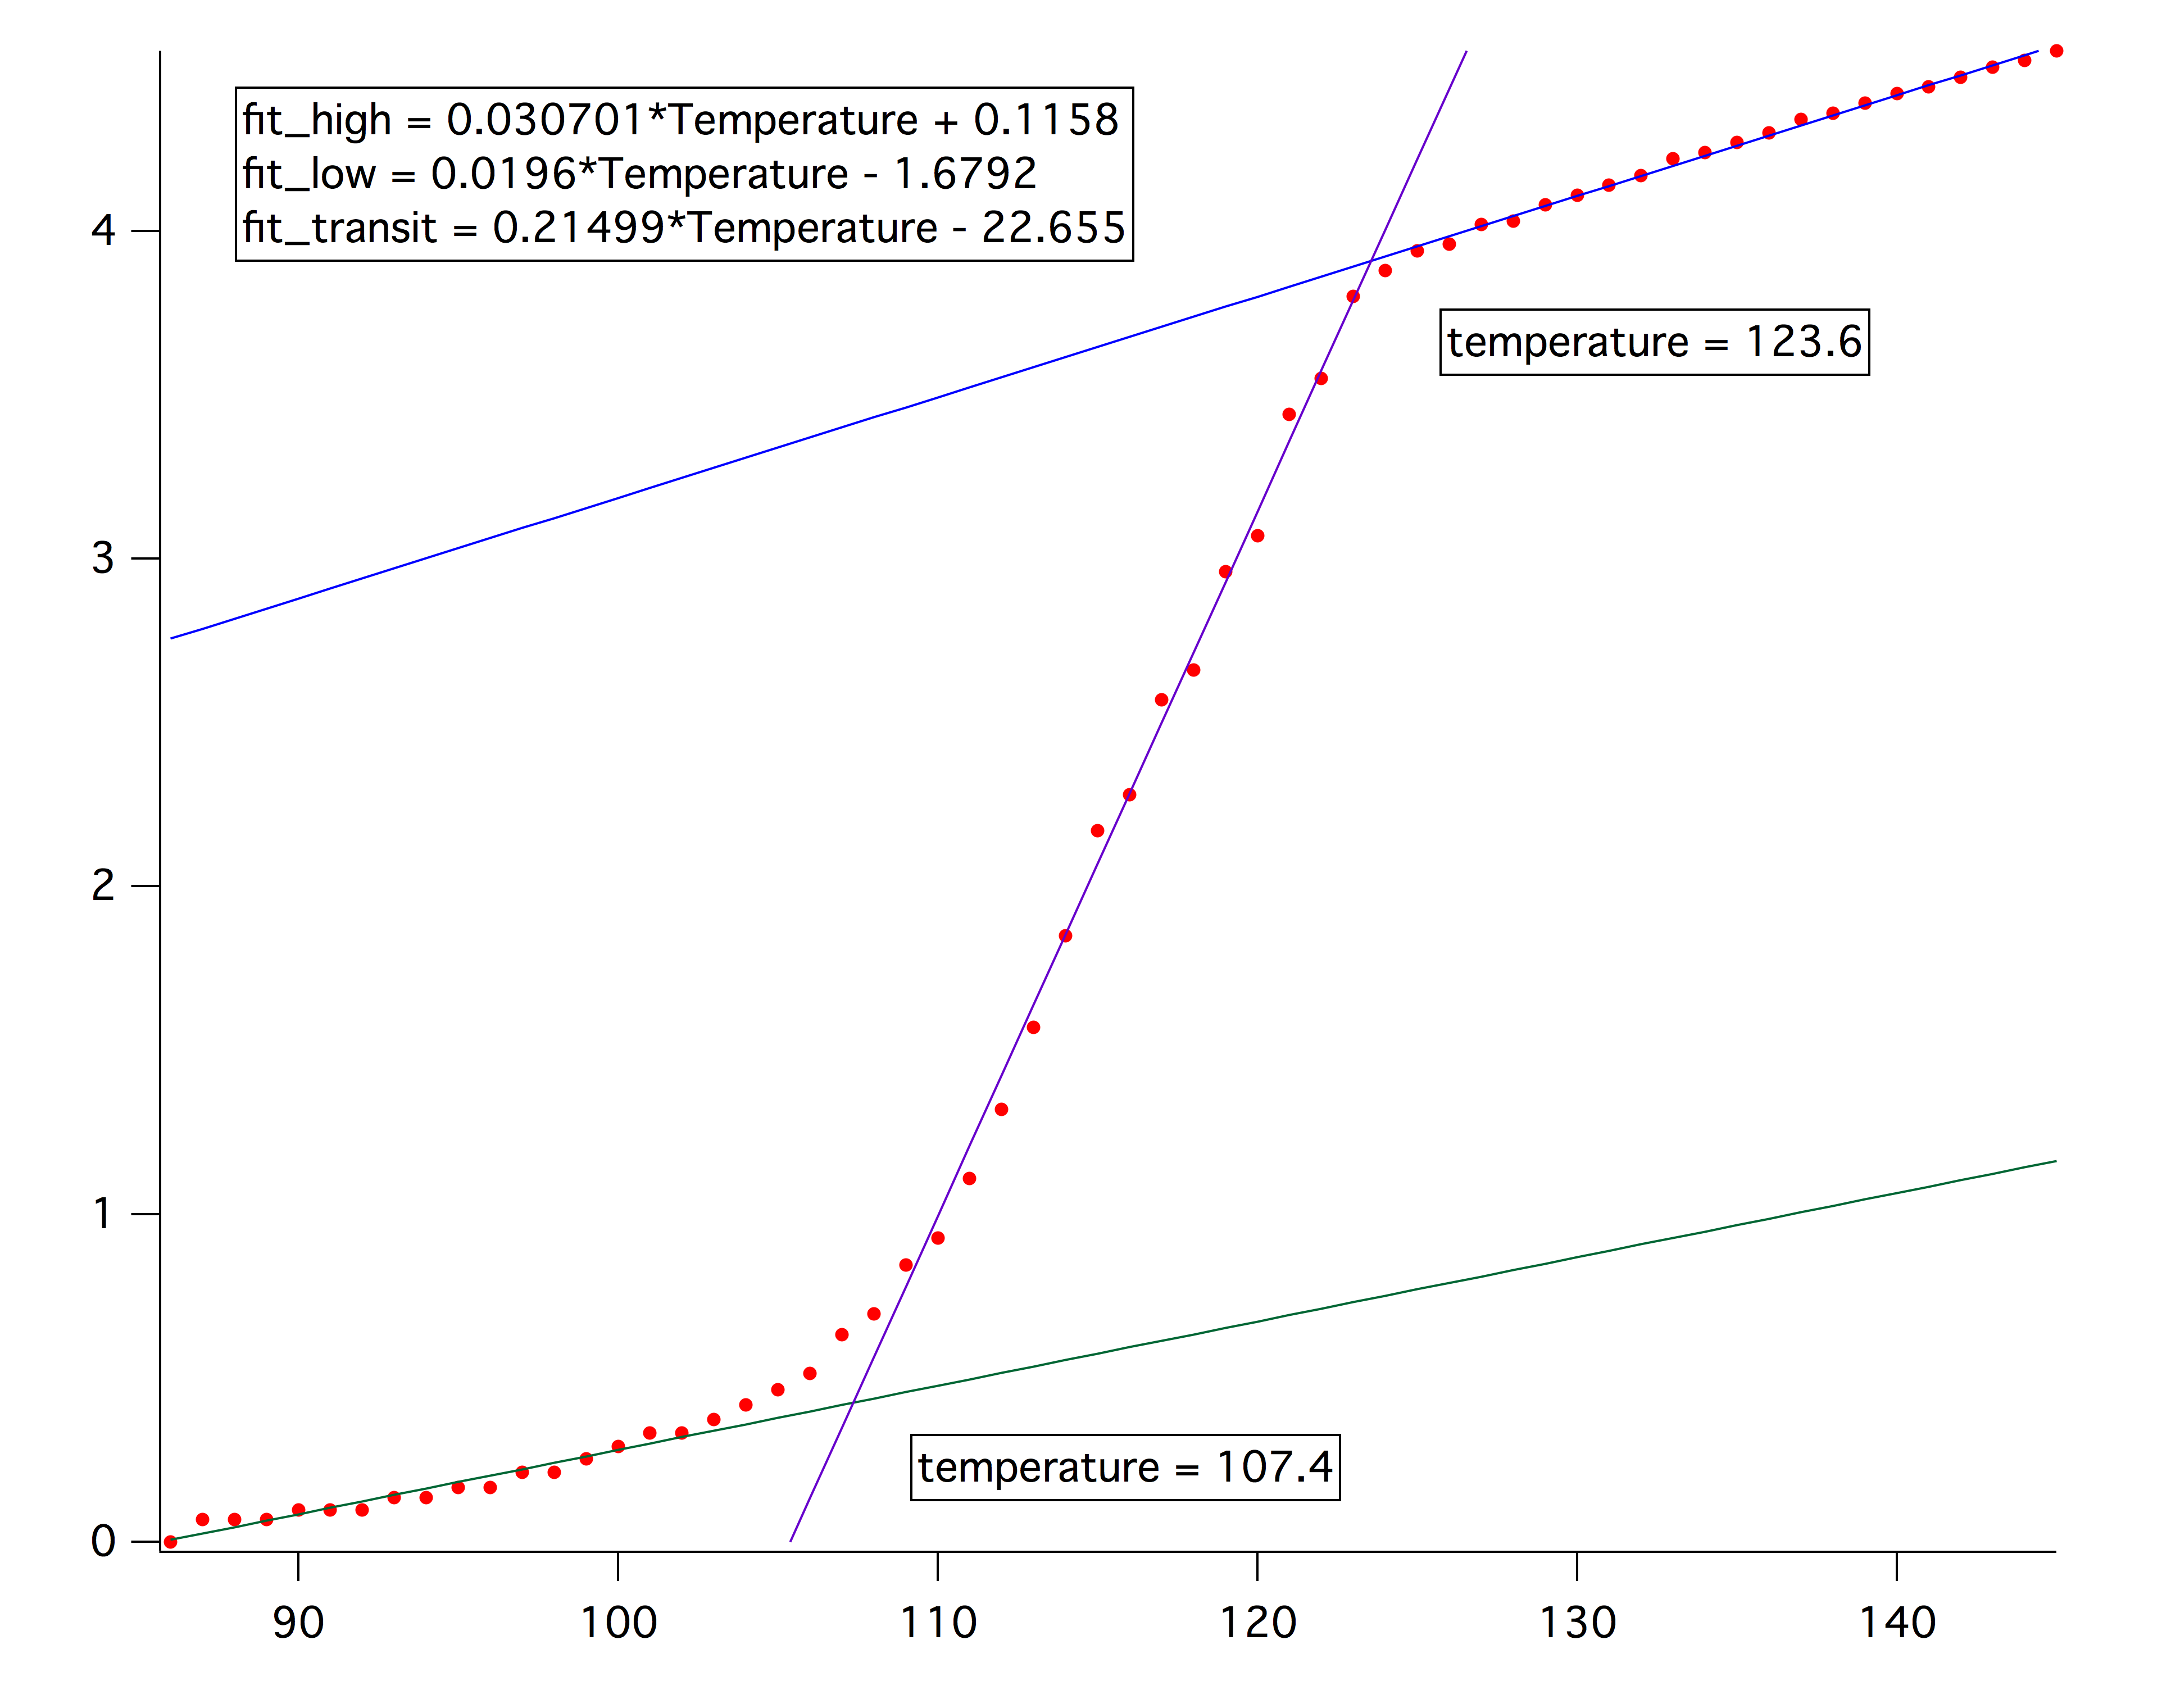
\includegraphics[width=11cm]{ybco100ma.png}
\caption{Analysis of data at current equal to 100mA}
\label{ybcoanalysis4}
\end{figure}

\end{appendix}

\end{document}
